% Options for packages loaded elsewhere
\PassOptionsToPackage{unicode}{hyperref}
\PassOptionsToPackage{hyphens}{url}
%
\documentclass[
  man,floatsintext]{apa7}
\usepackage{amsmath,amssymb}
\usepackage{iftex}
\ifPDFTeX
  \usepackage[T1]{fontenc}
  \usepackage[utf8]{inputenc}
  \usepackage{textcomp} % provide euro and other symbols
\else % if luatex or xetex
  \usepackage{unicode-math} % this also loads fontspec
  \defaultfontfeatures{Scale=MatchLowercase}
  \defaultfontfeatures[\rmfamily]{Ligatures=TeX,Scale=1}
\fi
\usepackage{lmodern}
\ifPDFTeX\else
  % xetex/luatex font selection
\fi
% Use upquote if available, for straight quotes in verbatim environments
\IfFileExists{upquote.sty}{\usepackage{upquote}}{}
\IfFileExists{microtype.sty}{% use microtype if available
  \usepackage[]{microtype}
  \UseMicrotypeSet[protrusion]{basicmath} % disable protrusion for tt fonts
}{}
\makeatletter
\@ifundefined{KOMAClassName}{% if non-KOMA class
  \IfFileExists{parskip.sty}{%
    \usepackage{parskip}
  }{% else
    \setlength{\parindent}{0pt}
    \setlength{\parskip}{6pt plus 2pt minus 1pt}}
}{% if KOMA class
  \KOMAoptions{parskip=half}}
\makeatother
\usepackage{xcolor}
\usepackage{color}
\usepackage{fancyvrb}
\newcommand{\VerbBar}{|}
\newcommand{\VERB}{\Verb[commandchars=\\\{\}]}
\DefineVerbatimEnvironment{Highlighting}{Verbatim}{commandchars=\\\{\}}
% Add ',fontsize=\small' for more characters per line
\usepackage{framed}
\definecolor{shadecolor}{RGB}{248,248,248}
\newenvironment{Shaded}{\begin{snugshade}}{\end{snugshade}}
\newcommand{\AlertTok}[1]{\textcolor[rgb]{0.94,0.16,0.16}{#1}}
\newcommand{\AnnotationTok}[1]{\textcolor[rgb]{0.56,0.35,0.01}{\textbf{\textit{#1}}}}
\newcommand{\AttributeTok}[1]{\textcolor[rgb]{0.13,0.29,0.53}{#1}}
\newcommand{\BaseNTok}[1]{\textcolor[rgb]{0.00,0.00,0.81}{#1}}
\newcommand{\BuiltInTok}[1]{#1}
\newcommand{\CharTok}[1]{\textcolor[rgb]{0.31,0.60,0.02}{#1}}
\newcommand{\CommentTok}[1]{\textcolor[rgb]{0.56,0.35,0.01}{\textit{#1}}}
\newcommand{\CommentVarTok}[1]{\textcolor[rgb]{0.56,0.35,0.01}{\textbf{\textit{#1}}}}
\newcommand{\ConstantTok}[1]{\textcolor[rgb]{0.56,0.35,0.01}{#1}}
\newcommand{\ControlFlowTok}[1]{\textcolor[rgb]{0.13,0.29,0.53}{\textbf{#1}}}
\newcommand{\DataTypeTok}[1]{\textcolor[rgb]{0.13,0.29,0.53}{#1}}
\newcommand{\DecValTok}[1]{\textcolor[rgb]{0.00,0.00,0.81}{#1}}
\newcommand{\DocumentationTok}[1]{\textcolor[rgb]{0.56,0.35,0.01}{\textbf{\textit{#1}}}}
\newcommand{\ErrorTok}[1]{\textcolor[rgb]{0.64,0.00,0.00}{\textbf{#1}}}
\newcommand{\ExtensionTok}[1]{#1}
\newcommand{\FloatTok}[1]{\textcolor[rgb]{0.00,0.00,0.81}{#1}}
\newcommand{\FunctionTok}[1]{\textcolor[rgb]{0.13,0.29,0.53}{\textbf{#1}}}
\newcommand{\ImportTok}[1]{#1}
\newcommand{\InformationTok}[1]{\textcolor[rgb]{0.56,0.35,0.01}{\textbf{\textit{#1}}}}
\newcommand{\KeywordTok}[1]{\textcolor[rgb]{0.13,0.29,0.53}{\textbf{#1}}}
\newcommand{\NormalTok}[1]{#1}
\newcommand{\OperatorTok}[1]{\textcolor[rgb]{0.81,0.36,0.00}{\textbf{#1}}}
\newcommand{\OtherTok}[1]{\textcolor[rgb]{0.56,0.35,0.01}{#1}}
\newcommand{\PreprocessorTok}[1]{\textcolor[rgb]{0.56,0.35,0.01}{\textit{#1}}}
\newcommand{\RegionMarkerTok}[1]{#1}
\newcommand{\SpecialCharTok}[1]{\textcolor[rgb]{0.81,0.36,0.00}{\textbf{#1}}}
\newcommand{\SpecialStringTok}[1]{\textcolor[rgb]{0.31,0.60,0.02}{#1}}
\newcommand{\StringTok}[1]{\textcolor[rgb]{0.31,0.60,0.02}{#1}}
\newcommand{\VariableTok}[1]{\textcolor[rgb]{0.00,0.00,0.00}{#1}}
\newcommand{\VerbatimStringTok}[1]{\textcolor[rgb]{0.31,0.60,0.02}{#1}}
\newcommand{\WarningTok}[1]{\textcolor[rgb]{0.56,0.35,0.01}{\textbf{\textit{#1}}}}
\usepackage{graphicx}
\makeatletter
\def\maxwidth{\ifdim\Gin@nat@width>\linewidth\linewidth\else\Gin@nat@width\fi}
\def\maxheight{\ifdim\Gin@nat@height>\textheight\textheight\else\Gin@nat@height\fi}
\makeatother
% Scale images if necessary, so that they will not overflow the page
% margins by default, and it is still possible to overwrite the defaults
% using explicit options in \includegraphics[width, height, ...]{}
\setkeys{Gin}{width=\maxwidth,height=\maxheight,keepaspectratio}
% Set default figure placement to htbp
\makeatletter
\def\fps@figure{htbp}
\makeatother
\setlength{\emergencystretch}{3em} % prevent overfull lines
\providecommand{\tightlist}{%
  \setlength{\itemsep}{0pt}\setlength{\parskip}{0pt}}
\setcounter{secnumdepth}{-\maxdimen} % remove section numbering
% Make \paragraph and \subparagraph free-standing
\ifx\paragraph\undefined\else
  \let\oldparagraph\paragraph
  \renewcommand{\paragraph}[1]{\oldparagraph{#1}\mbox{}}
\fi
\ifx\subparagraph\undefined\else
  \let\oldsubparagraph\subparagraph
  \renewcommand{\subparagraph}[1]{\oldsubparagraph{#1}\mbox{}}
\fi
\newlength{\cslhangindent}
\setlength{\cslhangindent}{1.5em}
\newlength{\csllabelwidth}
\setlength{\csllabelwidth}{3em}
\newlength{\cslentryspacingunit} % times entry-spacing
\setlength{\cslentryspacingunit}{\parskip}
\newenvironment{CSLReferences}[2] % #1 hanging-ident, #2 entry spacing
 {% don't indent paragraphs
  \setlength{\parindent}{0pt}
  % turn on hanging indent if param 1 is 1
  \ifodd #1
  \let\oldpar\par
  \def\par{\hangindent=\cslhangindent\oldpar}
  \fi
  % set entry spacing
  \setlength{\parskip}{#2\cslentryspacingunit}
 }%
 {}
\usepackage{calc}
\newcommand{\CSLBlock}[1]{#1\hfill\break}
\newcommand{\CSLLeftMargin}[1]{\parbox[t]{\csllabelwidth}{#1}}
\newcommand{\CSLRightInline}[1]{\parbox[t]{\linewidth - \csllabelwidth}{#1}\break}
\newcommand{\CSLIndent}[1]{\hspace{\cslhangindent}#1}
\ifLuaTeX
\usepackage[bidi=basic]{babel}
\else
\usepackage[bidi=default]{babel}
\fi
\babelprovide[main,import]{english}
% get rid of language-specific shorthands (see #6817):
\let\LanguageShortHands\languageshorthands
\def\languageshorthands#1{}
% Manuscript styling
\usepackage{upgreek}
\captionsetup{font=singlespacing,justification=justified}

% Table formatting
\usepackage{longtable}
\usepackage{lscape}
% \usepackage[counterclockwise]{rotating}   % Landscape page setup for large tables
\usepackage{multirow}		% Table styling
\usepackage{tabularx}		% Control Column width
\usepackage[flushleft]{threeparttable}	% Allows for three part tables with a specified notes section
\usepackage{threeparttablex}            % Lets threeparttable work with longtable

% Create new environments so endfloat can handle them
% \newenvironment{ltable}
%   {\begin{landscape}\centering\begin{threeparttable}}
%   {\end{threeparttable}\end{landscape}}
\newenvironment{lltable}{\begin{landscape}\centering\begin{ThreePartTable}}{\end{ThreePartTable}\end{landscape}}

% Enables adjusting longtable caption width to table width
% Solution found at http://golatex.de/longtable-mit-caption-so-breit-wie-die-tabelle-t15767.html
\makeatletter
\newcommand\LastLTentrywidth{1em}
\newlength\longtablewidth
\setlength{\longtablewidth}{1in}
\newcommand{\getlongtablewidth}{\begingroup \ifcsname LT@\roman{LT@tables}\endcsname \global\longtablewidth=0pt \renewcommand{\LT@entry}[2]{\global\advance\longtablewidth by ##2\relax\gdef\LastLTentrywidth{##2}}\@nameuse{LT@\roman{LT@tables}} \fi \endgroup}

% \setlength{\parindent}{0.5in}
% \setlength{\parskip}{0pt plus 0pt minus 0pt}

% Overwrite redefinition of paragraph and subparagraph by the default LaTeX template
% See https://github.com/crsh/papaja/issues/292
\makeatletter
\renewcommand{\paragraph}{\@startsection{paragraph}{4}{\parindent}%
  {0\baselineskip \@plus 0.2ex \@minus 0.2ex}%
  {-1em}%
  {\normalfont\normalsize\bfseries\itshape\typesectitle}}

\renewcommand{\subparagraph}[1]{\@startsection{subparagraph}{5}{1em}%
  {0\baselineskip \@plus 0.2ex \@minus 0.2ex}%
  {-\z@\relax}%
  {\normalfont\normalsize\itshape\hspace{\parindent}{#1}\textit{\addperi}}{\relax}}
\makeatother

\makeatletter
\usepackage{etoolbox}
\patchcmd{\maketitle}
  {\section{\normalfont\normalsize\abstractname}}
  {\section*{\normalfont\normalsize\abstractname}}
  {}{\typeout{Failed to patch abstract.}}
\patchcmd{\maketitle}
  {\section{\protect\normalfont{\@title}}}
  {\section*{\protect\normalfont{\@title}}}
  {}{\typeout{Failed to patch title.}}
\makeatother

\usepackage{xpatch}
\makeatletter
\xapptocmd\appendix
  {\xapptocmd\section
    {\addcontentsline{toc}{section}{\appendixname\ifoneappendix\else~\theappendix\fi\\: #1}}
    {}{\InnerPatchFailed}%
  }
{}{\PatchFailed}
\keywords{Parallel processing; writing; mixture models; language production; keystroke logging}
\usepackage{csquotes}
\usepackage{booktabs}
\usepackage{longtable}
\usepackage{graphicx}
\usepackage{array}
\usepackage{multirow}
\usepackage{float}
\usepackage{colortbl}
\usepackage{threeparttable}
\usepackage[normalem]{ulem}
\usepackage[utf8]{inputenc}
\usepackage{icomma}
\usepackage{pdflscape}
\newcommand{\blandscape}{\begin{landscape}}
\newcommand{\elandscape}{\end{landscape}}
\DeclareCaptionFormat{cont}{#1 (cont.)#2#3\par}
\makeatletter
\renewcommand{\paragraph}{\@startsection{paragraph}{4}{\parindent}%
  {0\baselineskip \@plus 0.2ex \@minus 0.2ex}%
  {-1em}%
  {\normalfont\normalsize\bfseries\typesectitle}}

\renewcommand{\subparagraph}[1]{\@startsection{subparagraph}{5}{1em}%
  {0\baselineskip \@plus 0.2ex \@minus 0.2ex}%
  {-\z@\relax}%
  {\normalfont\normalsize\bfseries\itshape\hspace{\parindent}{#1}\textit{\addperi}}{\relax}}
\makeatother

\ifLuaTeX
  \usepackage{selnolig}  % disable illegal ligatures
\fi
\usepackage{csquotes}
\IfFileExists{bookmark.sty}{\usepackage{bookmark}}{\usepackage{hyperref}}
\IfFileExists{xurl.sty}{\usepackage{xurl}}{} % add URL line breaks if available
\urlstyle{same}
\hypersetup{
  pdftitle={Typing in tandem: language planning in multi-sentence text production is fundamentally parallel},
  pdfauthor={Jens Roeser1, Rianne Conijn2, Evgeny Chukharev3, Gunn Helen Ofstad4, \& Mark Torrance1},
  pdflang={en-EN},
  pdfkeywords={Parallel processing; writing; mixture models; language production; keystroke logging},
  hidelinks,
  pdfcreator={LaTeX via pandoc}}

\title{Typing in tandem: language planning in multi-sentence text production is fundamentally parallel}
\author{Jens Roeser\textsuperscript{1}, Rianne Conijn\textsuperscript{2}, Evgeny Chukharev\textsuperscript{3}, Gunn Helen Ofstad\textsuperscript{4}, \& Mark Torrance\textsuperscript{1}}
\date{}


\shorttitle{Typing in tandem}

\authornote{

We are grateful for all authors who made their data available to us, in particular Nina Vandermeulen, Alessandra Rossetti, and colleagues, and Vibeke Rønneberg, Per Henning Uppstad, and colleagues at the Norwegian Reading National Centre, University of Stavanger . This work was supported by the National Science Foundation under Grant No.~2016868: \enquote{ProWrite: Biometric feedback for improving college students' writing processes.} and UKRI ESRC under Grant No.~ES/W011832/1: \enquote{Can you use it in a sentence?: Establishing how word-production difficulties shape text formation.}

Data and analysis scripts written in R and Stan can be found on OSF (\url{https://osf.io/z65dw/}; Roeser et al., 2024). For a tutorial on Bayesian mixture-model analysis in the context of keystroke data see \url{https://rpubs.com/jensroes/mixture-models-tutorial}.

Parts of this work have been shared through conference presentations, namely at the SIG writing conference in Paris, France (2024) and in Umea, Sweden (2022), and at EARLI SIG Online Measurements in Southampton, UK (2022).

The authors made the following contributions. Jens Roeser: Conceptualisation, Data curation, Formal analysis, Funding acquisition, Investigation, Methodology, Project administration, Software, Visualisation, Writing -- original draft, Writing -- review \& editing; Rianne Conijn: Conceptualisation, Investigation, Writing -- original draft, Writing -- review \& editing; Evgeny Chukharev: Funding acquisition, Investigation, Resources, Project administration, Software, Supervision; Gunn Helen Ofstad: Investigation, Resources; Mark Torrance: Conceptualisation, Data curation, Formal analysis, Funding acquisition, Investigation, Methodology, Resources, Supervision, Visualisation, Writing -- original draft, Writing -- review \& editing.

Correspondence concerning this article should be addressed to Jens Roeser, 50 Shakespeare St, Nottingham NG1 4FQ. E-mail: \href{mailto:jens.roeser@ntu.ac.uk}{\nolinkurl{jens.roeser@ntu.ac.uk}}

}

\affiliation{\vspace{0.5cm}\textsuperscript{1} Department of Psychology, Nottingham Trent University, United Kingdom\\\textsuperscript{2} Human-Technology Interaction Group, Eindhoven University of Technology, The Netherlands\\\textsuperscript{3} Department of English, Iowa State University, Iowa\\\textsuperscript{4} Educational Sciences and Humanities, University of Stavanger, Norway}

\abstract{%
Classical serial models view the process of producing a text as a chain of discrete pauses, during which the next span of text is planned, and bursts of activity during which this text is output onto the page or computer screen. In contrast, semi-parallel models of writing assume that planning is not complete at production onset and operates in parallel with execution. Across six datasets from participants composing multi-sentence texts we instantiated these assumptions in two sets of Bayesian mixed effects models: (1) single-distribution models as assumed by the serial processing account, and (2) a finite (two-distribution) mixture model as assumed by the parallel processing account. We analysed interkey intervals at before-sentence, before word, and within word transitions. Model comparisons demonstrated strong evidence in favour of the parallel view across all datasets. When pausing occurred, sentence initial pauses were longer than word initial pauses which is consistent with the idea that larger linguistic edges are associated with higher level planning. However, we found -- across populations -- that interkey intervals at word and even at sentence boundaries were often too rapid to permit planning of what was written next. Our results cannot be explained by the serial processing but are in line with the semi-parallel view of writing.
}



\begin{document}
\maketitle

Translating ideas into language involves a sequence of processes starting with communicative intent, proceeding through generation of a message, retrieving appropriate lexical items, deciding with which part of the message to start the utterance (which, depending on theoretical viewpoint (Bock \& Ferreira, 2014; Wheeldon \& Konopka, 2023), is determined by syntactic requirements of our language) and then retrieving orthographic and / or phonological codes, these are finally submitted to the motor programs that output speech, key or pen-strokes or signs (Olive, 2014; Van Galen, 1991; Wheeldon \& Konopka, 2023).

The coordination of these processes in writing is arguably more demanding than in spoken language. This is because writing requires spelling retrieval, which may or may not be mediated by phonology, and the motor planning and execution required to press keys or move a pen. Pen control and typing skills are later-developing and more effortful than those required to articulate language sounds in speech and, possibly as a consequence, written output rate is typically slower (for a recent review see Kandel, 2023). Consequently mentally buffering of linguistic plans prior to output is likely to play a greater role in writing than in speech.

Written communication is also less time constrained: speaking comes with fluency requirements because hesitating during speech has a communicative effect (e.g. Clark \& Fox Tree, 2002). There is therefore stronger pressure to plan ahead in speech than in writing (Roeser et al., 2019; Torrance \& Nottbusch, 2012). Indeed writers can pause when they wish -- even in the middle of a word -- and for how long they want without compromising communication. Written production of multi-sentence texts -- composing an argumentative essay, for example -- therefore involves a combination for relatively fluent production bursts followed by pauses (Chenoweth \& Hayes, 2001).

The study reported in this paper compares statistical models that instantiate two different theories of how cognitive planning processes are coordinated in writing. Through the analysis of 6 different datasets from writers of different ages and competencies composing multi-sentence texts, we compare these statistical models and therefore the cognitive models of text production onto which they map. Also, we evaluate competing predictions of these models by revisiting the often-reported finding that edges of larger linguistic units are associated with longer pauses (Conijn et al., 2019; Flower \& Hayes, 1981; Matsuhashi, 1981; Wengelin, 2006). In what follows we first summarise previous research that has explored pause patterns in spontaneous text production. We then introduce two possible cognitive frameworks in which these can be interpreted. Finally we argue that analysis of pause-patterns at linguistic edges is necessary to permit differentiation between these two theories.

We focus on data form spontaneous text production (see Gernsbacher \& Givón, 1995) for the following three reasons: First, text production such as essay, argumentative, and narrative writing in response to a writing brief or topic statement is a natural environment for text production (Dux Speltz et al., 2022; Dux Speltz \& Chukharev-Hudilainen, 2021; Vandermeulen et al., 2023). Second, since the emergence of keystroke-logging software such as InputLog (Leijten \& Van Waes, 2013) recording keystroke data during free text composition has become widely used among writing researchers and led to a rapidly expanding timecourse literature; for a recent special issue see Conijn and Torrance (2023).\footnote{Social Science Citation Index reports 40 journal papers that describe research exploring composition processes using keystroke logging methods in 2022, compared to 26 in 2017 to 2019, and 7 in 2014 to 2016.} These data are therefore important for contemporary theories of writing and freely available for statistical modelling and machine learning (Conijn et al., 2019; Conijn, 2020). Third, spontaneous text production is not constrained in the same way as it would be in experiments in which text is elicited in response to picture stimuli (Damian \& Stadthagen-Gonzalez, 2009; Meulemans et al., 2022; Nottbusch, 2010; Roeser et al., 2019) or is copied (Roeser, De Maeyer, et al., 2024; Van Waes et al., 2019, 2021). Instead the content-determination processes are free to run entirely internally, without the need to consult an image or a text that must be copied.\footnote{Also, pauses in text production do not reflect visual encoding of the stimulus (although possibly reflect looking back during writing which we will return to in the discussion).}

Time intervals between adjacent keystrokes during typing vary as a function of various factors. Explaining the factors that influence the duration of inter-keystroke intervals (interkey intervals) requires a theory of how the various processes that transform intent into keypresses are structured. Planning what to say and how to say it may be serial. This means that the processing sequence operates one unit at a time. Under this theory, planning of the next language unit can only start when the previous unit has been fully processed, from communicative intention to completion of the written output. Therefore interkey intervals represent periods when the writer is planning what to write next: interkey interval will be longer at linguistic edges where planning scopes over larger text spans and their duration represents the time necessary to complete that planning (Alves \& Limpo, 2015; Hayes, 2012; Kaufer et al., 1986; Matsuhashi, 1981; Schilperoord, 2002).

This serial account is consistent with the frequent finding that the average interkey interval duration immediately before larger linguistic units is longer compared to smaller linguistic units. For example, in spontaneous text the mean pause duration before a writer starts a sentence has typically been reported to be longer than before a mid-sentence word and these are, in turn, longer than between mid-word key presses (Deane \& Zhang, 2015; Mohsen, 2021; Spelman Miller, 2006; Spelman Miller et al., 2008; Torrance, Rønneberg, et al., 2016; Wengelin, 2002; Xu \& Qi, 2017). This is understood as being due to time needed to plan message and syntax for the next sentence, which is added to the time required to prepare the upcoming word, and the motor planning required to produce the first keystroke of that word (Baaijen et al., 2012; Medimorec et al., 2017; Medimorec \& Risko, 2017; Roeser et al., 2019). However this account is not consistent with two other sets for findings:

First, writers and speakers can in principle plan utterances in full for one or multiple sentences before beginning to output words. However this is not what people typically do: utterances are not fully formed at production onset. Instead, syntax and lexical content and even details of the message itself are planned as the emergent result of a real-time process. For speech it is well known that the pre-planning duration depends -- among other factors -- on the need to avoid intra-sentential hesitations; speakers have a preference towards minimising language pre-planning depending on the extent to which upcoming words can be planned in parallel to production (Griffin, 2003; e.g. Levelt \& Meyer, 2000; Wheeldon \& Konopka, 2023). For writing, there is evidence that the time to keystroke / pen onset increases when a sentence starts with a more complex sentence-initial phrases similar as in speech (Damian \& Stadthagen-Gonzalez, 2009; Nottbusch, 2010; Roeser et al., 2019). For example, in Roeser et al. (2019) participants described moving arrays of images in simple utterances such as \emph{A and the B moved above the C} that either started with a conjoined noun phrase (i.e.~\emph{A and the B moved}) or a simple noun (i.e., \emph{A moved above the B and the C}). Importantly while the overall complexity of the utterance (in terms of length, number of phrases and noun) was held constant, sentences that started with a conjoined noun phrase increased the time to typing onset (and speech onset). This is not what one would expect if writers plan sentences in full before production onset. In fact, eye-movement data reported in Torrance and Nottbusch (2012) and Roeser et al. (2019) demonstrate that writers do not plan the lexical form of the utterance beyond the first noun before production onset (similar to speech Griffin, 2001, 2003), although there was evidence that lexical pre-planning of the second noun (i.e.~\emph{the B}) was more likely for conjoined noun phrases, i.e.~when the second noun was part of the same phrase as the first noun.

Second, even though the average sentence-initial interkey interval tends to be longer, they still tend to be very rapid. For example, Medimorec and Risko (2017) found that, in undergraduate students' writing on familiar topics 71\% of sentence-initial interkey intervals were less than 1 seconds in duration. Also Rønneberg et al. (2022) reported that sentence-initial hesitations are rare, with over 50\% of sentences preceded by very short pauses (around 430 msecs) and a mean of 1.2 seconds for the remainder of pauses. For comparison, these short pauses are less than mean written naming response latency for single objects (Torrance et al., 2018) in a similar population. Longer pauses in the remainder were similar to response latencies for short sentences when describing arrays of images (Roeser et al., 2019), also in a similar population. Despite the fact that writers can in principle pause when they want to, written composition is often remarkably fluent. The fact that these very short sentence-initial pauses exist, and in fact are quite common, is not consistent with the assumption that planning of the upcoming sentence is started and finished in the period between completion of the previous sentence and starting to write the next.

If utterances are not planned in full prior to writing onset, how is it possible that at least for reasonably competent writers composting multi-sentence texts typically occurs remarkably fluently, with very few hesitations. The two examples above and similar findings point towards much of the mental activity associated with composition, including the relatively complex processing required to plan sentences, occurring as a result of a cascade of processes that operates partly in parallel and largely without executive control. Consistent with general trends in language processing theory (Bock \& Ferreira, 2014; Chang et al., 2006; Dell et al., 2007), several researchers have argued that the processes associated with written production run at least in part in parallel (Bonin et al., 2012; Crump \& Logan, 2010; Olive, 2014; Roux et al., 2013; Van Galen, 1991). Van Galen (1991), for example, argued for a cascade of modular processes each responsible for a specific transformation (semantic, syntactic, and so forth), with processing occurring as soon as information from the immediately upstream process becomes available (Christiansen \& Chater, 2016). Buffers provide transient storage at each processing level to accommodate unsynchronised output rates: when lower level processes lag behind higher level processes buffers allow fingers to catch up with message and language processing. Under this account when writers move from one sentence to another without hesitation this is due to then having completed required planning for the next sentence in parallel with output of the the sentence that they have just completed.

This semi-parallel cascaded account of the composition process therefore gives a rather different understanding of inter-keystroke intervals. Interkey intervals result from one of two sets of underlying mental processes. When upstream processes output at a rate equal to or faster than can be used for finger movement planning, then interkey intervals are determined just by the time needed for executing finger movements (i.e.~just by processing below the last buffer in the processing cascade). However if one or more upstream processes provide output more slowly, then interkey intervals are determined just by time taken to complete upstream processes and not on finger movement. These two distinct data-generating processes mean that interkey intervals are a mixture of two distributions, one associated with the very rapid processing necessary for actioning keystrokes, and another that forms as a result of delays resulting from some combination of processing at the semantic, syntactic, lexical, or orthographic level not being complete at the time of the immediately preceding keystroke (Roeser, De Maeyer, et al., 2024). The parallel account provides an explanation for why writers sometimes hesitate before sentence (or word) onset, but often do not. This is not because in some cases sentences are not planned, or planning was postponed until after sentence onset, but that this planning was completed in parallel with previous output.

Capturing this understanding of interkey intervals requires statistical models that are premised on more than one data-generating process. These models have been adopted in a number of psycholinguistic studies. For example, in language comprehension, Vasishth and colleagues (Vasishth, Jäger, et al., 2017; Vasishth, Chopin, et al., 2017) demonstrated convincingly that some phenomena in online sentence comprehension observed in reading times are captured better by statistical models that assume that the underlying mental process that generates reading data is in fact a mixture of two process expressed as two distributions in the statistical implementation. In the context of written production Roeser, De Maeyer, et al. (2024) demonstrated\footnote{For similar approaches see Almond et al. (2012), Baaijen et al. (2012), Chenu et al. (2014), Guo et al. (2018), Hall et al. (2022), Li (2021), and Van Waes et al. (2021).} how models that allow the possibility of two underlying data-generating processes revealed two separate distributions when participants were copy-typing sentences or lists of words that are more pronounced for tasks with challenging orthographic sequences but reduced down to just one distribution in a tapping task where participants merely pressed two keys repeatedly as quickly as possible (e.g.~\enquote{dkdkdkdk}). As argued by the authors, copy-typing underlies a similar cascade of processes as free text composition: copy-typing provides a typing context that is constrained to visual encoding of the target string and the retrieval of motor codes for letter combinations. For relatively experienced writers, visual encoding is likely to happen in parallel to writing (De Smet et al., 2018); hesitations occur when motor codes, for example for low frequency bigrams, were not retrieved in time (Roeser, De Maeyer, et al., 2024). However composition tasks are different from copy tasks: in copy tasks but not in spontaneous text production, content generation and grammatical encoding is artificially constrained to particular sequences of letter bigrams, words or sentences, and copy-typing involves a combination of visual encoding of the target string and mental buffering prior to the activation of motor codes. Typing hesitations in the context of copy-typing may -- to some extent -- reflect not just production but also, and possibly largely, visual encoding. Text composition, in contrast, provides data from the free generation of words and full sentences that is not dependent on a visually presented text stimulus. For these reasons our research extends the analysis of keystroke data using a mixture model approach to data from spontaneous text production.

\hypertarget{present-study}{%
\subsection{Present Study}\label{present-study}}

In the study that is presented in this paper we use Bayesian hierarchical models of keystroke intervals -- similar to Roeser, De Maeyer, et al. (2024) -- to identify whether the semi-parallel view of writing generalises to contexts in which participants compose texts. On the basis of these statistical models of text composition, we appraise to what extent linguistic edges (sentence and word boundaries) are associated with different pausing behaviours as frequently suggested in the literature (Ailhaud et al., 2016; Ailhaud \& Chenu, 2017; Chukharev-Hudilainen et al., 2019; Conijn et al., 2019; Mohsen, 2021; Torrance, Rønneberg, et al., 2016; Wengelin, 2002).

The hypotheses are as follows: if the preparation of the upcoming production unit happens entirely at the corresponding linguistic edge as predicted by the serial account, and not in parallel to production, key-transition intervals can statistically be modelled as a function of the associated transition location. In other words, we expect interkey intervals to be proportionally longer at before-sentence locations compared to before-word locations compared to within-word locations. This is because transitions before larger linguistic units are associated with processing that involves higher levels of representation. The semi-parallel cascading view, in contrast, assumes that although interkey intervals at larger linguistic edges might be longer, it is in principle possible that writers do not (always) pause to plan their text but plan in parallel to writing. In other words, statistical models of the pause-and-burst view of written production do not capture that planning can operate, to some extent, in parallel to the output of the written production. Therefore, a statistical model that captures writing as a cascade of processes must account for the possibility that hesitations occur to some extent probabilistically across the entire text although some linguistic locations such as larger linguistic edges are associated with a higher pausing probability. We hypothesise that the statistical model of the parallel view provides a better out-of-sample generalisation than the implementation of the serial model of writing in the context of unconstrained spontaneous text composition. We tested these models across 6 datasets.

For each dataset we evaluated four Bayesian statistical models. The first three models were premised on the (traditional) single-distribution understanding of interkey intervals. These models are consistent with the assumption that processing leading to a keystroke is fundamentally serial. In the first model we assumed the interkey intervals were drawn from a Gaussian (normal)distribution. In the second we assumed a log-Gaussian distribution. In both cases, consistent with previous studies that have modelled inter-keystroke intervals, we assumed equal variance across different linguistic edges (within words, at word boundaries, and at sentence boundaries). To provide a fairer comparison with the two-distribution model that followed we tested a third unequal variance model that allowed intervals associated with higher-order linguistic edges to have greater variability.

The fourth model was premised on the assumption that the processing that results in a keystroke runs, in part, in parallel with preceding output. As we have discussed, this model assumes two data-generating processes. We therefore followed the finite (two-distribution) mixture-modelling approach described by Roeser, De Maeyer, et al. (2024). This model assumes that interkey intervals result from a mixture of: (1) uninhibited activation flow into motor programmes and (2) interruptions at higher levels that cause delays in this information flow. Therefore interkey intervals are not directly and sufficiently determined by transition location -- as in the serial account -- but are also associated with different probabilities that a hesitation occurs.

\hypertarget{methods}{%
\section{Methods}\label{methods}}

We analysed interkey intervals from six existing studies in which participants composed spontaneous, multi-sentence texts in response to writing prompts. The datasets include samples from populations with various writing experience and languages (e.g.~young / L2 writers, students) performing different writing tasks (e.g.~essays, syntheses). Datasets from a variety of different populations of writers and writing tasks were deliberately chosen to challenge our modelling approach and to test to what extent pausing patterns generalise across writing contexts.

This study was not preregistered.

\hypertarget{data-sets}{%
\subsection{Data sets}\label{data-sets}}

Six datasets with keystroke data from free text production were used for analysis. An overview can be found in Table \ref{tab:datasets}; descriptions below. Datasets used are C2l1 (Rønneberg et al., 2022), CATO (Torrance, Rønneberg, et al., 2016), GE2 (Ofstad Oxborough \& Torrance, 2011), SPL2 (Torrance et al., n.d.), LIFT published in Vandermeulen, Steendam, et al. (2020) and described in Vandermeulen, De Maeyer, et al. (2020), and PLanTra published in Rossetti and Van Waes (2022b) and described in Rossetti and Van Waes (2022a).

\begin{landscape}

\begin{table}[tbp]

\begin{center}
\begin{threeparttable}

\caption{\label{tab:datasets}Datasets in brief.}

\footnotesize{

\begin{tabular}{p{1.5cm}p{2.75cm}p{1.75cm}p{2.25cm}p{1.75cm}p{1.75cm}p{.5cm}p{2.5cm}p{1.75cm}p{2cm}}
\toprule
Dataset & \multicolumn{1}{c}{Source} & \multicolumn{1}{c}{Keylogger} & \multicolumn{1}{c}{Writing task} & \multicolumn{1}{c}{Words in text$^a$} & \multicolumn{1}{c}{Age} & \multicolumn{1}{c}{N} & \multicolumn{1}{c}{Sample} & \multicolumn{1}{c}{Country} & \multicolumn{1}{c}{Language}\\
\midrule
C2L1 & Rønneberg et al. (2022) & EyeWrite & Argumentative essay & 128.5 (52.9) & 11.8 (0.47) & 126 & 6th graders & Norway & Norwegian\\
CATO & Torrance et al. (2016) & EyeWrite & Expository essay & 288 (119) & 16.9 (0.88) & 52 & Secondary school students (dyslexic, non dyslexic) & Norway & Norwegian\\
GE2 & Torrance and Ofstad (n.d) & EyeWrite & Argumentative essay & 540 (141) & 19.1 (1.4)$^c$ & 45 & Undergraduate students & UK & English\\
LIFT & Vandermeulen, Steendam, et al. (2020) & InputLog & Synthesis of several printed sources$^b$ & 374 (56)$^d$ & 16.7 (1.5) & 658 & Secondary school students & The Netherlands & Dutch\\
PLanTra & Rossetti and Van Waes (2022b) & InputLog & Paraphrase technical text$^b$ & 295 (79) & 23 (2.7) & 47 & Master students & Belgium & English (L2)\\
SPL2 & Torrance et al. (n.d.) & CyWrite & Argumentative essay & 668 (301) & 20.6 (1.62) & 39 & Undergraduate students & USA & English\\
\bottomrule
\addlinespace
\end{tabular}

}

\begin{tablenotes}[para]
\normalsize{\textit{Note.} $^a$Mean number of words in the final text; standard deviations in parentheses. $^b$Reading activity was marked in the dataset and removed before analysis. $^c$Estimated from a similar sample from the same population. $^d$Estimated based on the number of characters in the final product following Brysbaert et al. (2021).}
\end{tablenotes}

\end{threeparttable}
\end{center}

\end{table}

\end{landscape}

In C2L1 Norwegian 6th graders composed argumentative essays. In CATO upper Norwegian secondary students with and without dyslexia composed expository texts either normally or with masked letters to prevent writers reading their unfolding text. In SPL2 undergraduate students produced argumentative essays in their first language (L1; English) and in a second language L2 (Spanish) in which they were able to compose text but in which their mastery fell well behind their first language. Order of language (L1 / L2) and two writing prompts were counterbalanced. The LIFT data are from pre-university students producing argumentative and informative text syntheses on four topics each. The PLanTra data contains data from Master students in Business and Economics simplifying texts on sustainability, before and after receiving either online instruction on how to apply plain language principles to sustainability content or an online instruction exclusively on the topic of sustainability. The GE2 data are from Undergraduate students producing two argumentative essays on general-knowledge topics in either masked text or normal writing conditions, with masking, topic and order counterbalanced.

For C2L1, CATO, and GE2, keystroke data were captured using EyeWrite (Simpson \& Torrance, 2007; Torrance, 2012). LIFT and PLanTra data were captured using InputLog (Leijten \& Van Waes, 2013; Van Waes et al., 2019, 2021) and SPL2 data were collected using CyWrite (Chukharev-Hudilainen et al., 2019).

\hypertarget{data-extraction}{%
\subsection{Data extraction}\label{data-extraction}}

From the keystroke data we extracted interkey intervals between adjacent keys at locations that have been identified repeatedly in previous research as locations where observed mean interkey intervals (or counts of interkey intervals over a predetermined threshold) have tended to vary substantially (e.g. Chukharev-Hudilainen et al., 2019; De Smet et al., 2018; Torrance, Rønneberg, et al., 2016) and are detailed in Table \ref{tab:keyloc}. In particular we analysed the interkey intervals that resulted in the insertion of a character that started a new sentence (before-sentence transition); interkey intervals that started a new word (other than those at the beginning of a sentence; before-word transitions); and transitions between characters within words all transitions. At before-sentence locations, interkey intervals were timed to the shift keypress that resulted in the capitalization of the first key for most data sets (CATO, C2L1, SPL2, GE2) but were timed to the character key press in the PLanTra and LIFT datasets (i.e.~the duration included the time to perform the capitalising shift keypress); we return to this difference in the Results section. Transitions that occurred at the very start of the text or at the beginning of a paragraph were not treated as before-sentence transitions and were removed from the analysis. Importantly we also removed transitions that were followed by an editing operation. We therefore just modelled the times between keypresses in ongoing production.

\begin{table}[tbp]

\begin{center}
\begin{threeparttable}

\caption{\label{tab:keyloc}Transition location classification. The final text in all cases was "The cat meowed. Then it slept."}

\footnotesize{

\begin{tabular}{p{3cm}p{5cm}p{6cm}}
\toprule
Transition type & \multicolumn{1}{c}{Description} & \multicolumn{1}{c}{Example}\\
\midrule
Within word & Transitions between any letter & T$^{\wedge}$h$^{\wedge}$e c$^{\wedge}$a$^{\wedge}$t m$^{\wedge}$e$^{\wedge}$o$^{\wedge}$w$^{\wedge}$e$^{\wedge}$d. T$^{\wedge}$h$^{\wedge}$a$^{\wedge}$t[bsp][bsp]e$^{\wedge}$n i$^{\wedge}$t s$^{\wedge}$l$^{\wedge}$e$^{\wedge}$p$^{\wedge}$t.\\
Before word & Keypress after space followed by any letter & The $^{\wedge}$cat $^{\wedge}$meowed. That[bsp][bsp]en $^{\wedge}$it $^{\wedge}$slept.\\
Before sentence & Keypress following a space preceding any letter & The cat meowed. $^{\wedge}$That[bsp][bsp]en it slept.\\
\bottomrule
\addlinespace
\end{tabular}

}

\begin{tablenotes}[para]
\normalsize{\textit{Note.} $'^{\wedge}$' marks transition location; [bsp] represents backspace.}
\end{tablenotes}

\end{threeparttable}
\end{center}

\end{table}

We removed participants that did not complete all conditions in studies with within-participant factors (reducing the number of participants to 343 for LIFT data, and 41 participants for PLanTra data). We removed participants that produced fewer than 10 sentences (LIFT: 109 participants; PLanTra: 3 participants; SPL2: 1 participant). We further removed keystroke intervals that were too short to represent intentional typing (\(\le\) 50 msecs, see Gentner et al., 1980; Rumelhart \& Norman, 1982) or were of a length where such that they were unlikely to be associated with ongoing text production (\(\ge\) 30 secs); percentages can be found in Table \ref{tab:datareduction}. From the remaining data we randomly sampled a maximum of 100 observations per participant, condition, and transition location (when more than 100 were available). This was done to reduce the computation time of the Bayesian models required to complete sampling. For the LIFT data set we reduced the number of participants to 100 because the total sample was substantially larger than for the other datasets. Because the LIFT data set included the largest number of writing tasks, we sampled 50 observations per condition, location and participant which would otherwise exceed the computational resources available to us. The number of keystroke data used in the analysis can be found in Table \ref{tab:datareduction}.

\begin{table}[bp!]

\begin{center}
\begin{threeparttable}

\caption{\label{tab:datareduction}Data reduction. Shown are the percentage of extreme data that were removed and the percentage of randomly sampled data that were analysed by transition location (`--` if all data were included). Standard error in parentheses.}

\begin{tabular}{lrrrrr}
\toprule
 \multicolumn{1}{c}{ } & \multicolumn{2}{c}{Extreme values in \%} & \multicolumn{3}{c}{Data analysed in \%} \\
\cmidrule(r){1-1} \cmidrule(r){2-3} \cmidrule(r){4-6}
Dataset & \multicolumn{1}{c}{$\le$ 50 msecs} & \multicolumn{1}{c}{$\ge$ 30 secs} & \multicolumn{1}{c}{within word} & \multicolumn{1}{c}{before word} & \multicolumn{1}{c}{before sentence}\\
\midrule
C2L1 & 0.19 (0.1) & 0.074 (0.063) & 35 (2.6) & 85 (1.8) & --\\
CATO & 0.65 (0.15) & 0.023 (0.016) & 15 (0.95) & 49 (2.2) & --\\
GE2 & 2.2 (0.17) & 0.0072 (0.0055) & 6.2 (0.43) & 23 (1.4) & --\\
LIFT & 2.6 (0.16) & 0.0048 (0.0038) & 3.2 (0.22) & 13 (0.86) & 99 (0.15)\\
PLanTra & 2.5 (0.41) & 0.04 (0.031) & 9.7 (0.64) & 37 (1.9) & --\\
SPL2 & 2.3 (0.2) & 0.028 (0.016) & 5.7 (0.39) & 23 (1.4) & --\\
\bottomrule
\end{tabular}

\end{threeparttable}
\end{center}

\end{table}

\hypertarget{statistical-modelling}{%
\subsection{Statistical modelling}\label{statistical-modelling}}

We analysed keystroke data in a series of four Bayesian mixed-effects models. An overview of all models can be found in Table \ref{tab:models}. Full modelling details can be found in Appendix \ref{statistical-models} but we summarised the most relevant properties in this section.

The first three models -- models M1, M2, and M3 -- were single-distribution models consistent with the serial account. They were single distribution models, with fixed effects for each combination of transition location and dataset-specific manipulations. Models M1 (Gaussian) and M2 (log-Gaussian) are consistent with standard models used in the literature and therefore serve as baseline models. For model M3 we relaxed the equal-variance assumption for transition locations, thus allowing transition locations on larger linguistic boundaries to assume a larger standard deviation; see Appendix \ref{statistical-models} for rationale.

\begin{table}[tbp]

\begin{center}
\begin{threeparttable}

\caption{\label{tab:models}Model overview. All models included by-participant random effect and study-specific manipulations.}

\begin{tabular}{lp{13cm}}
\toprule
Models & \multicolumn{1}{c}{Description}\\
\midrule
\textbf{Serial} & \\
\ \ \ M1 & Single Gaussian model with effects of transition location.\\
\ \ \ M2 & Single distribution log-Gaussian model equivialent to M1.\\
\ \ \ M3 & Equivalent to M2 but with different variance components for each transition location (unequal variance).\\
\textbf{Parallel} & \\
\ \ \ M4 & Two-distributions mixture of a log-Gaussian for fluent interkey intervals and another wider log-Gaussian for hesitant / disfluent interkey intervals; the distribution of hesitant interkey intervals assumes -- similar to M3 -- different values for transition locations. The mixing weight of these distributions capture the relative number of disfluent transitions for each transition location.\\
\bottomrule
\end{tabular}

\end{threeparttable}
\end{center}

\end{table}

Model M4 is a two-distribution mixture model consistent with the parallel cascading account. This model assumes that keystroke data result from a combination of two data generating processes; these models are referred to as finite mixture models in the literature (Gelman et al., 2014; MacLahlan \& Peel, 2000). Both single-distribution models and the two-distribution mixture model capture that processing difficulty at higher levels of activation leads to longer pauses but only the two-distribution model captures that planning-related pauses may occur at any interkey interval, even mid-word, and that planning may not be reflected in sentence or word-initial pauses when planning happens in parallel to output. In other words, instead of assuming that there is one process that shifts the distribution of transition durations for larger linguistic edges, we allow for the possibility that key-transitions at larger linguistic edges are more likely to reflect processing delays but the cognitive system does not obligate planning to occur before sentences or words. This is achieved by modelling interkey intervals as coming from a weighted mixture of two distributions associated with two different states, illustrated in equation \ref{eq:bimodcon2}:

\begin{enumerate}
\def\labelenumi{\arabic{enumi}.}
\item
  Information from upstream mental processes can flow into keystrokes without interruption at intermediate levels. These fluent keystroke transitions are merely constrained by a person's ability to move their finger. Fluent interkey intervals (i.e.~typing speed) are captured by the \(\beta\) parameter. \(\beta\) is represented in both log-Gaussian distributions in equation \ref{eq:bimodcon2} referring to the same unknown parameter.
\item
  Any interruption at upstream levels of mental representation delays the information flow reflected in a resulting lag between keystroke intervals, for example when words or their spelling could not be retrieved in time. The slowdown for such hesitations is captured by \(\delta\) and its frequency by the mixing proportion \(\theta\). The slowdown \(\delta\) was allowed to vary by transition locations because hesitations at larger linguistic units are likely to be associated with higher level planning which causes longer delays in the output. The \(\delta\) parameter was constrained to be positive, so that it captures how much longer hesitant interkey intervals are in addition to \(\beta\).
\end{enumerate}

\begin{equation}
\begin{aligned}
\label{eq:bimodcon2}
\text{iki}_{i} \sim\text{ } & \theta_\text{location[i], participant[i]} \times \text{log}\mathcal{N}(\beta + \delta_\text{location[i]} + u_\text{participant[i]}, \sigma_{e'_\text{location[i]}}^2) + \\
  & (1 - \theta_\text{location[i], participant[i]}) \times \text{log}\mathcal{N}(\beta + u_\text{participant[i]}, \sigma_{e_\text{location[i]}}^2)\\
\text{where: } & u_\text{participant} \sim \mathcal{N}(0, \sigma_\text{p}^2) \\
\text{constraint: } & \delta, \sigma_{e}^2, \sigma_\text{e'}^2, \sigma_\text{p}^2>0\\
        & \sigma_{e'}^2 > \sigma_{e}^2\\
        & 0 < \theta < 1
\end{aligned}
\end{equation}

The first line of equation \ref{eq:bimodcon2} represents the distribution of hesitant interkey intervals that include the \(\delta\) parameter presenting the slowdown for hesitant transitions; the second line represents the distribution of fluent -- uninterrupted -- interkey intervals that is characterised by \(\beta\) which is also present in the first file. Either of these two distributions is associated with the mixing proportion \(\theta\) that ranges between 0 and 1. \(\theta\) was parameterised here to represent the probability that an interkey interval is associated with the distribution of hesitant transitions. This probability is inversely related to the mixing weight of the distribution of fluent transitions by \(1-\theta\) . In other words, a larger weight for either distribution inevitably means a lower weight for the other. We call this parameter the probability of hesitant interkey intervals. When a parameter is allowed to vary by transition location (levels: before sentence, before word, within word), this was indicated as subscript; similar for participants. For example, \(\theta_\text{location[i], participant[i]}\) means that the mixing proportion \(\theta\) is allowed to take on a different value for both the transition location and participant associated with the \(i^\text{th}\) keystroke interval \(i \in 1 \ldots N\) where \(N\) is the total number of keystroke intervals. Because the hesitation probability was allowed to vary by participants as well as location type, we included a hyper-parameter for the mixing proportion \(\theta\) for each transition location.

As with model M3, M4 allowed the variance associated with the key-intervals indicated as \(\sigma_{e'}^2\) to vary by transition location. Further each of the two distributions in M4 had its own variance constrained such that the variance associated with the distribution of hesitant keystrokes \(\sigma_{e'}^2\) was larger than the distribution of fluent keystroke intervals \(\sigma_{e}^2\). This is important because slower human behaviour similar to hesitant keystroke transitions is generally known to be associated with a larger variability (Schöner, 2002; Wagenmakers \& Brown, 2007; Wing \& Kristofferson, 1973). Model M4 and all other models included a random intercepts term \(u_\text{participants}\) for participants which is constrained to be distributed around 0 with an unknown standard deviation, i.e.~\(\mathcal{N}(0, \sigma_\text{p}^2)\), hence indicating participant specific deviations from the average typing speed \(\beta\).

All models were implemented in the Bayesian framework (Gelman et al., 2014; McElreath, 2016). In the present analysis, we used weakly informative priors to aid model convergence by constraining the parameter space to plausible values (see e.g. Lambert, 2018; McElreath, 2016). Also, as the sample size of most of our datasets is large, weakly informative priors have no or a negligible effect on the posterior. Stan code for mixture models was based on Roeser, De Maeyer, et al. (2024; see also Vasishth, Chopin, et al., 2017; Vasishth, Jäger, et al., 2017) and can be found on OSF (Roeser, Conijn, et al., 2024); for a tutorial see \href{rpubs.com/jensroes/mixture-models-tutorial}{https://rpubs.com/jensroes/mixture-models-tutorial}.\footnote{The R (R Core Team, 2020) package rstan (Stan Development Team, 2018) was used to interface with the probabilistic programming language Stan (Carpenter et al., 2016) which was used to implement all models. Models were run with 20,000 iterations on 3 chains with a warm-up of 10,000 iterations and no thinning. Model convergence was confirmed by the Rubin-Gelman statistic (\(\hat{R}\) = 1) (Gelman \& Rubin, 1992) and inspection of the Markov chain Monte Carlo chains. The predictive performance of our models was compared using leave-one-out cross-validation (Sivula et al., 2020; Vehtari et al., 2015, 2017).}

To compare the out-of-sample predictive performance of our models we used leave-one-out cross-validation based on Pareto smoothed importance-sampling (Vehtari et al., 2015, 2017). Predictive performance was estimated as the sum of the expected log predictive density (\(\widehat{elpd}\)) and compared by the difference between models \(\Delta\widehat{elpd}\). We also summarised this difference as normalised over its standard error \(\mid\frac{\Delta\widehat{elpd}}{\text{SE}}\mid\), the \emph{z}-score of the difference between models (Sivula et al., 2020). Similar to other cross-validation techniques, the advantage of leave-one-out cross-validation is that more complex models -- models with more parameters -- are penalised to prevent overfit.

\hypertarget{results}{%
\section{Results}\label{results}}

\hypertarget{model-comparisons}{%
\subsection{Model comparisons}\label{model-comparisons}}

The differences in the predictive performance of models for all datasets are shown in Table \ref{tab:loos}. For all six dataset the two-distributions mixture model (M4) provided greater predictive performance than all three single-distribution models. Differences in predictive performance (\(\Delta\widehat{elpd}\)) between models M4 and the nearest competing single-distribution model (M3) ranged between {[}18, 40{]} standard errors, indicating a substantially higher predictive performance for the two-distributions model. Among the single distribution models we found higher predictive performance for the unequal variance model and the lowest predictive performance for the single distribution Gaussian. Comparisons showing the fit of model predictions to the data can be found in Appendix \ref{fit-to-data} and echo the findings in Table \ref{tab:loos}. Data predicted by the two-distribution mixture model closely align with the observed data; data predicted by single distribution Gaussian models showed an inferior fit to the data.

\begin{table}[tbp]

\begin{center}
\begin{threeparttable}

\caption{\label{tab:loos}Model comparisons. Models were compared incrementally from the simplest to the most complex model. Comparison are shown with the distribution type of the model with the higher predictive performance. A negative difference in $\Delta\widehat{elpd}$ indicates higher predictive performance for the more complex model; standard error shown in parentheses.}

\small{

\begin{tabular}{p{1.75cm}p{4cm}p{4.25cm}p{3.5cm}}
\toprule
Dataset & Mixture of two log-Gaussians (M3 -- M4) & Single log-Gaussian (unequal variance; M2 -- M3) & Single log-Gaussian (M1 -- M2)\\
\midrule
C2L1 & -1,637 (72) & -785 (60) & -37,517 (798)\\
CATO & -1,782 (75) & -1,299 (71) & -37,673 (881)\\
GE2 & -2,427 (92) & -2,312 (89) & -38,843 (616)\\
LIFT & -5,105 (127) & -2,111 (99) & -74,851 (1,624)\\
PLanTra & -2,384 (90) & -1,381 (80) & -33,823 (526)\\
SPL2 & -1,181 (64) & -1,713 (69) & -28,717 (418)\\
\bottomrule
\addlinespace
\end{tabular}

}

\begin{tablenotes}[para]
\normalsize{\textit{Note.} $\Delta\widehat{elpd}$ = difference in predictive performance -- estimated as expected log pointwise predictive density}
\end{tablenotes}

\end{threeparttable}
\end{center}

\end{table}

\hypertarget{transition-location-effect}{%
\subsection{Transition location effect}\label{transition-location-effect}}

Figure \ref{fig:mixmodel} illustrates the mixture model results for every dataset: for each interkey interval we obtained two posterior probability distributions, one associated with fluent transitions between keys and another for interkey intervals where upstream difficulty resulted in hesitant interkey intervals. The hesitation probability -- the probability of interkey intervals associated with hesitations -- is indicated as the height of the distribution shown in yellow (on the right of each panel). The transition locations are characterised by the hesitation parameters: as we illustrate the mixture model, the distributions of fluent transitions -- indicated in grey -- are constant across transition location (within each dataset) but their height differs as the probability of fluent interkey intervals is the inverse of the height of hesitant interkey intervals; i.e.~\(1 - \theta\). Within-word interkey intervals have a negligibly small hesitation probability barely visible in the visualisation. Hesitations before words and sentences are both roughly equally likely than fluent transitions. In other words, half of the time participants did not pause before a word or sentence; we explore this below. However, when hesitations occurred, these are longer at before-sentence interkey intervals compared to before word interkey intervals. The slowdown for hesitant interkey intervals -- represented earlier as \(\delta\) -- is the distance between the distribution of fluent interkey intervals (\(\beta\)) shown in grey and the distribution of hesitant interkey intervals shown in yellow.

\begin{figure}

{\centering \includegraphics{manuscript_files/figure-latex/mixmodel-1} 

}

\caption{Mixture model plot for each transition location. Shown are the distributions for both mixture components (fluent and hesitant interkey intervals) and their weighting. Interkey intervals are shown in seconds on log scaled intervals.}\label{fig:mixmodel}
\end{figure}

Figure \ref{fig:mixmodel} highlighted how model parameters relate to each other in pairs of distributions but to compare the effect of transition location on model parameters we need to compare the posterior distribution of the three parameters of interest individually. Therefore Figure \ref{fig:crossstudypost2} visualises the same posterior as Figure \ref{fig:mixmodel} but expressed directly in terms of posterior probability distributions of the individual mixture-model parameters. These are shown for all datasets by transition location. Although models were fitted with all dataset-specific conditions, we aggregated the posterior across conditions\footnote{We aggregated across pre and post tests for the PLanTra dataset as well as genre and topic of the LIFT data set. We demonstrate in Appendix \ref{pre-post-test-plantra} and \ref{genre-effect-lift}, respectively, that there is negligible evidence for differences between these conditions.}, and excluded conditions that might confound comparisons\footnote{We removed the masked writing condition in the GE2 and CATO, the dyslexic group in the CATO data set, and L2 writing in the SPL2 data set. There was evidence for L2 writing effects (see Appendix \ref{l2-effect-spl2}); evidence for marking effects was weak (see Appendix \ref{masking-effect-cato-ge2}).}. For posteriors of all conditions within datasets see Appendix \ref{posterior-parameter-estimates}. The resulting posterior allows us to examine differences and similarities associated with transition locations for all datasets. In particular we can see how transition location in the text is associated with hesitant interkey intervals and hesitation probability. For completeness we also report the estimate for fluent interkey intervals.

\begin{figure}

{\centering \includegraphics{manuscript_files/figure-latex/crossstudypost2-1} 

}

\caption{Mixture model parameter estimates across studies. Distributions of parameter estimates are represented as posterior mean and 95\% probability interval (PI). Interkey-interval duration measures are shown in msecs and hesitation probability is shown in proportions. Estimates for the CATO dataset were calculated for the non-dyslexic group, unmasked condition; also the GE2 estimtes represent the unmasked condition; SPL2 estimates are for the L1 group.}\label{fig:crossstudypost2}
\end{figure}

Figure \ref{fig:crossstudypost2} shows largely the same patterns (with caveats) for all datasets. We summarise the evidence for differences between transitions locations in Table \ref{tab:loceffectconbf}. We found that hesitations were more frequent -- higher hesitation probability -- before words than within words (BFs \textgreater{} 100 for all datasets) but only for half of the datasets hesitation durations were longer (GE2: BF = 27; PLanTra: BF = 56; SPL2: BF = 9.1; negligible evidence for C2L1: BF = 0.1; CATO: BF = 0.2; LIFT: BF = 0.4). Hesitations were equally likely before sentences and words (C2L1 and CATO: BFs = 0.7; PLanTra: BF = 0.3; LIFT: BF = 1.6; except for GE2 and SPL2; both BFs \textgreater{} 100) but longer (all BFs \textgreater{} 100, except for C2L1: BF = 1.11 and LIFT = 0.5). Full results and parameter estimates can be found in Appendix \ref{transition-location-effect-1}.

\begin{table}[tbp]

\begin{center}
\begin{threeparttable}

\caption{\label{tab:loceffectconbf}BFs for the effect of transition location on interkey intervals shown for the hesitation duration and hesitation probability. Comparisons for the CATO dataset were calculated for the non-dyslexic group, unmasked condition; also the GE2 estimtes represent the unmasked condition; SPL2 estimates are for the L1 group.}

\begin{tabular}{lp{3cm}p{3cm}p{3cm}p{3cm}}
\toprule
 & \multicolumn{2}{c}{Hesitation duration} & \multicolumn{2}{c}{Hesitation probability} \\
\cmidrule(r){2-3} \cmidrule(r){4-5}
Dataset & before sentence vs word & before vs within word & before sentence vs word & before vs within word\\
\midrule
C2L1 & 1.11 & 0.07 & 0.68 & > 100\\
CATO & > 100 & 0.2 & 0.67 & > 100\\
GE2 & > 100 & 26.78 & > 100 & > 100\\
LIFT & 0.5 & 0.41 & 1.61 & > 100\\
PLanTra & > 100 & 55.53 & 0.28 & > 100\\
SPL2 & > 100 & 9.07 & > 100 & > 100\\
\bottomrule
\addlinespace
\end{tabular}

\begin{tablenotes}[para]
\normalsize{\textit{Note.} BF = evidence in favour of the alternative hypothesis over the null hypothesis calculated using the Savage-Dickey method (Dickey et al., 1970; Wagenmakers et al., 2010). BFs greater than 3 indicate moderate evidence, greater than 10 strong evidence, and greater than 30 very strong evidence for a statistically meaningful effect (Jeffreys, 1961; Lee \& Wagenmakers, 2014). A BF smaller than 0.33 suggests evidence in favour of a null effect (Dienes, 2014) and a BF around 1 is inconclusive evidence.}
\end{tablenotes}

\end{threeparttable}
\end{center}

\end{table}

To reiterate, for most datasets we found that pauses before sentences are longer but not always more likely than before words (except for SPL2 and GE2). In fact, LIFT showed some indication that pauses were less likely before sentences than words. This is interesting because it is generally believed that pausing behaviour is associated with linguistic boundaries such that more and longer pauses are predicted for interkey intervals at larger linguistic edges (see Introduction section). It is less clear in which contexts pre-sentence pausing is more likely than pausing before words.

Differences between datasets could, to some extent, be explained by the fact that two datasets (PLanTra, LIFT) defined before-sentence transitions as the sum of transitions between space, shift and the sentence-initial character, while the remaining data sets measured before-sentence transitions as the interval between space key and shift. To test to what extent complex key combinations affects the parameter estimates, we addressed this possibility for the SPL2 dataset and showed that including the character following the shift key substantially increased the hesitation probability for sentence-initial transitions (BFs \textgreater{} 100) but it did not affect the duration hesitant interkey intervals (BFs \textless{} 0.3); see Appendix \ref{key-combination-effect}. This conflicts with the earlier finding that before-sentence hesitations were not more likely than before-word hesitations for datasets that did include the character following shift (PLanTra, LIFT). In other words, patterns in our results cannot be explained on the basis of how sentence-initial key transitions were operationalised.

Finally, Figure \ref{fig:crossstudypost2} highlights that fluent interkey intervals in two datasets (C2L1, CATO) were substantially longer than for other datasets. This is presumably reflecting that these data were sampled from the youngest and least experienced population of writers in our data pool. Interestingly, however, hesitation duration and hesitation probability followed the same patterns as the majority of datasets.

\hypertarget{discussion}{%
\section{Discussion}\label{discussion}}

The classical serial view (Flower \& Hayes, 1980) characterises composing spontaneous multi-sentence text as a sequence of planning and execution cycles. Text is therefore produced as a series of production bursts bounded by pauses. The parallel model of writing, in contrast, sees planning, at least in competent writers, as occurring to a large extent in parallel with output (Olive, 2014). The implication of this for observation of writing timecourse -- of inter-key intervals as writers compose text -- is that pause duration doesn't necessarily correlate with planning necessary for next output. We implemented these two views in Bayesian statistical models, hierarchical single-distribution models capturing the serial view, and a two-distribution mixture model capturing predictions about patterning of interkey intervals under the assumption of semi-parallel upstream processing. Fitting these models with six sets of keystroke data from free text production tasks -- with a total of 953 participants producing 5,223,280 interkey intervals -- we have found compelling and consistent statistical evidence in favour of the parallel view. In all cases, the predictive performance of the two-distribution mixture-models (consistent with the parallel view of writing) outperformed the single-distribution models.

The two distribution model assumes two data generating processes, one associated with the immediate demands of motor planning required for the production of a keystroke, and one that captures all upstream processing from message to abstract letter representation. A direct implication of parallel, cascaded processing is that the distribution over interkey intervals is not additive -- it is not a combination of time to motor plan plus time for upstream processing. The interval between keypresses is \emph{either} determined by motor execution \emph{or} by processing that occurred upstream of motor execution (in cases where provision of output from the upstream processes lags behind the rate at which it can be output by the fingers). Under a serial account -- where all planning necessary for production of next-text occurs in the interkey interval immediately before output of -- interkey interval will be the sum of times for each processing step required for generation of that text. Both accounts predict longer mean interkey intervals at higher-order text edges (interkey intervals greater before sentences than before mid-sentence words, and before mid-sentence words than before mid-word characters). This has been consistently observed in a number of previous studies (Deane \& Zhang, 2015; Mohsen, 2021; Spelman Miller, 2006; Spelman Miller et al., 2008; Torrance, Rønneberg, et al., 2016; Wengelin, 2002; Xu \& Qi, 2017). However, the serial account does not permit the possibility of a distribution of short interkey intervals at higher-order edges: It strongly predicts that \emph{all} sentence boundaries will be associated with interkey intervals that are longer than those required just for the motor planning of the next character. Under the parallel-processing account it is very likely that some -- perhaps a large majority -- of interkey intervals before sentences will be longer. However there will be a distinct subset that is drawn from a distribution associated just with interkey intervals necessary for motor execution.

This is what we found. At all linguistic edges we found a distribution of interkey intervals at durations to motor execution at durations substantially below a threshold that might plausibly be necessary for, for example, lexical / orthographic retrieval (Grudin \& Larochelle, 1982; Ostry, 1983; Terzuolo \& Viviani, 1980; Van Waes et al., 2021). For mid-word interkey intervals, as might be expected, the mixture model predicted that the vast majority of interkey intervals fall within this distribution. Across the six datasets that we sampled, the central tendency for the duration of mid-word interkey intervals was broadly similar to mean mid-word interkey intervals observed in previous studies. Importantly, however, these short interkey intervals were also present at higher-order text edges. Across all datasets we found, at minimum, a non-trivial minority of sentence-initial interkey intervals were sampled from the short distribution (i.e.~with durations that could only be associated with motor execution). In two cases -- for writers sampled in the PLanTra and Lift datasets -- the majority of interkey intervals fell within this distribution. Thus, although as might be expected there was a considerably increased tendency for longer interkey intervals at higher order boundaries: Planning associated with planning a new sentence is, probabilistically, much more likely to spill beyond output of the previous sentence and therefore affect duration of the sentence-initial interkey interval. However the presence of a non-trivial proportion of interkey intervals with a duration that is inconsistent with anything other than motor execution can only be explained with recourse to theories that permit preparation in parallel with preceding output.

Our results showed that the hesitation probabilities are largely identical before sentences and before words, which suggests that writers frequently plan the next word and even sentence in parallel to production -- consistent with the parallel view of writing -- which mitigates the need to pause to plan up-coming linguistic information.

This parallelism was evident even in the youngest writers in our data pool (C2L1; mean age: 11.8 years). As might be expected for children who compose predominantly by handwriting and whose typing skills will still be developing, motor execution rate (mean duration of fluent transitions) was substantially slower compared to the more experienced typists in other datasets. In all other respects, however, findings for this dataset were similar to that of other datasets and consistent with parallel processing. A two-distribution mixture model provided best fit to these data. At both before-word and before-sentence locations a non-trivial number of interkey intervals were within the short distribution - i.e.~at durations too short to permit lexical retrieval or syntactic planning. Probability of longer intervals was greater before-sentence and before-word transitions compared to mid-word transitions. This is interesting because, for example, Olive (2014) described a parallel model that operates in a serial fashion for inexperienced or struggling writers, explained on the basis of task demands that reduce the ability to plan in parallel to processing which leads to a serialisation of planning units. However, the results presented in this paper suggest that pausing behaviour in young writers largely mirror results from more experienced writers: Pauses were both equally long and likely at before-word and before-sentence transitions but more likely compared to mid-word transitions. Also for L2 writers (PLanTra) we observe pausing patterns that do not resemble a serialised writing process as evidenced by a large number of fluent transitions at word and sentence boundaries.

We observed two more differences among datasets that are worth highlighting. Writers sampled in the GE2 and SPL2 datasets were more likely to pause before sentences than before words (see also Medimorec \& Risko, 2017; Wengelin, 2002). In the remaining datasets from writers who were either younger (and not educationally-selected) or writing in second language, hesitation was equally probable pre-word and pre-sentence. This is most readily attributed simply to increased demands of lexical and / or orthographic processing in these samples.

Second, pauses at before-sentence locations were not always longer than before words or mid-word; specifically there were two exceptions: (1) sentence-initial hesitations were not longer than word-initial hesitation for the C2L1 dataset possibly because these sample of young inexperienced writers tend to use a more localised word-level planning strategy for text production. (2) pause durations did not vary across transition locations in the LIFT dataset. The absence of a difference could be explained as specific to the writing task because, in synthesis, there is less need for planning novel contents and text structure: the structure of one the source texts might have been used during synthesis (\enquote{structural isomorphism,} Hidi \& Anderson, 1986). However, the results of the PLanTra dataset rule out this possibility: there was evidence for longer hesitations at larger linguistic edges for a text simplification task that also does not require planning of contents.

We are, therefore, interpreting the superior predictive performance of the two-distribution mixture model as strong evidence for parallelism in written composition. An alternative, more prosaic explanation might be that two-distribution models outperform single distributions simply because they estimate more parameters; two distributions will always provide better fit than one distribution models due just to overfitting. There are two related reasons not to prefer this explanation. First, the cross-validation methods that we used to compare model predictive performance favour more parsimonious models and are therefore robust to overfitting. Second, in the analysis described in Appendix \ref{simulation} we directly tested the hypothesis that modelling data randomly sampled from a single log-normal distribution as a two-distribution mixture will provide better fit than modelling as a single distribution. We found that the two-distribution mixture model was successful at uncovering the parameter values of the data generated with a two-distributions mixture process; we observed the same for the single-distribution model applied to the data generated with a single distribution process. Parameters were not successfully uncovered when we switched model type and dataset. Cross-validation rendered a substantially higher predictive performance for the mixture model compared to the single-distribution model for data sampled from a two-distributions mixture process, but not when applied to data based on a single-distribution process. Therefore we can rule out the possibility that the statistical support for the two-distributions mixture-models can be explained on the basis of their larger number of parameters (i.e.model overfitting).

Throughout this paper we have been attributing longer (second-distribution) interkey intervals to spill-over from upstream pre-motor processing that could not be completed in its entirety in parallel with previous output. These longer inter-key intervals may also, on occasion, be associated with activity that is initiated after the preceding process and is entirely bounded by the duration of the pause. We are thinking here specifically of the tendency, particularly at higher order text boundaries, for writers to glance back into their existing text (Alamargot et al., 2010; Beers et al., 2010; Chukharev-Hudilainen et al., 2019; De Smet et al., 2018; Torrance et al., n.d.; Van Waes et al., 2010). Torrance, Johansson, et al. (2016) found that lookbacks appear with a frequency of 45\% before sentences, 12\% before words and 5\% within words of which 36\% were associated with sustained reading but mostly less patterned forward and backward saccades between words (\enquote{hopping,} see also Chukharev-Hudilainen et al., 2019). There are broadly two reasons why writers might look back into their existing text.\footnote{Eye movement between key presses in writing-from-sources tasks will also be associated with reading source texts. Note, however, that for two datasets (PLanTra, LIFT) that involved writing from sources, we removed transitions that were made when the source (rather than the writing document) was in focus.} Lookback may be associated with monitoring just-produced text for errors. In the present study we excluded interkey intervals that preceded deletion or cursor movement, and also intervals at timescales that might be associated with strategic reviewing of large spans of text (e.g., reading text-already-written from top to bottom). However it may be that some longer intervals were associated with monitoring that failed to find errors that needed correcting. A second function for lookback may be to support planning next-text (Hayes, 1996; Johansson et al., 2010; Torrance, Johansson, et al., 2016). The preceding text, and particularly the preceding sentence, is a rich source of cues to support retrieval of both content and lexical items necessary to prepare what to write next. This will become particularly important where upstream processing lags behind the rate at which it can be output, and one or more of the buffers necessary to resolve this \enquote{temporal friction} (Van Galen, 1991) becomes overloaded. Comparison of conditions unmasked and masked text conditions in the CATO and GE2 datasets -- conditions in which writers could and could not read the text that they had already produced -- suggested that, if anything, proportion of longer interkey intervals at sentence boundaries was greater when text was masked (details in Appendix \ref{masking-effect-cato-ge2}). This finding is consistent both with lookback being only a minor contributor to interkey interval and, where it does occur, serving a rapid memory-refresh function. There is also some evidence, at least in the context of handwritten production, that eye movements back into already-written text themselves occasionally occur in parallel with output (Alamargot et al., 2007).

The findings we report in this paper are, we argue, the first robust evidence for parallelism in written composition of multi-sentence texts. The conclusion that text production processes are fundamentally parallel will not come as a surprise to most researchers. Parallel processing has a long history in theories of speech production (Chang et al., 2006; Dell, 1986; Dell et al., 1999; Dell \& O'Seaghdha, 1992; Garrett, 1975; Levelt, 1989). The transitory nature of activation and storage during fluent spoken production prevent, for example, generating phonological code a long time before it is required to drive articulation (Christiansen \& Chater, 2016). Spoken production is \enquote{just-in-time}. Perhaps because, at least in principle, there is not the same push to fluency in written production -- in principle writers can pause at any point with no detriment to communication -- writing extended text has tended to be seen as fundamentally serial, with pauses to prepare next-text followed by bursts of output during which this is executed (Flower \& Hayes, 1980). Our findings suggest that this is not the case. The language production processes that underlie text production follow the same just-in-time principle as speech.

\hypertarget{conclusion}{%
\section{Conclusion}\label{conclusion}}

The parallel view of writing, in contrast to the serial view, claims that writers do not necessarily pause to plan the upcoming language unit but plan in parallel with output. In this paper we have demonstrated, across six datasets, that statistical models premised on a parallel-processing understanding of planning in written composition outperform models premised on serial processing. We also found that interkey intervals across word and even sentence boundaries are frequently at timescales that are not consistent with planning of upcoming linguistic information. This pattern was found to be largely consistent for populations with different levels of writing experience and languages (e.g.~young / L2 writers, students) and across different composition tasks. Our argument that written composition -- a very common form of language production -- is a largely parallel process is probably uncontroversial. However, the findings we presented in this paper constitute the first robust evidence in support of this claim.

\newpage

\hypertarget{references}{%
\section{References}\label{references}}

\begingroup

\hypertarget{refs}{}
\begin{CSLReferences}{1}{0}
\leavevmode\vadjust pre{\hypertarget{ref-ailhaud2018variations}{}}%
Ailhaud, E., \& Chenu, F. (2017). Variations of chronometric measures of written production depending on clause packaging. \emph{CogniTextes}, \emph{17}. \url{https://doi.org/10.4000/cognitextes.992}

\leavevmode\vadjust pre{\hypertarget{ref-ailhaud2016developmental}{}}%
Ailhaud, E., Chenu, F., \& Jisa, H. (2016). A developmental perspective on the units of written {F}rench. In J. Perera, M. Aparici, E. Rosado, \& N. Salas (Eds.), \emph{Written and spoken language development across the lifespan: Essays in honour of {Liliana Tolchinsky}} (pp. 287--305). Springer. \url{https://doi.org/10.1007/978-3-319-21136-7_17}

\leavevmode\vadjust pre{\hypertarget{ref-Alamargot2007}{}}%
Alamargot, D., Dansac, C., Chesnet, D., \& Fayol, M. (2007). {Parallel Processing Before and After Pauses: A Combined Analysis of Graphomotor and Eye Movements During Procedural Text Production}. In M. Torrance, L. Van Waes, \& D. Galbraith (Eds.), \emph{Writing and cognition} (pp. 11--29). BRILL. \url{https://doi.org/10.1163/9781849508223_003}

\leavevmode\vadjust pre{\hypertarget{ref-alamargot2010using}{}}%
Alamargot, D., Plane, S., Lambert, E., \& Chesnet, D. (2010). Using eye and pen movements to trace the development of writing expertise: Case studies of a 7th, 9th and 12th grader, graduate student, and professional writer. \emph{Reading and Writing}, \emph{23}(7), 853--888.

\leavevmode\vadjust pre{\hypertarget{ref-almond2012preliminary}{}}%
Almond, R., Deane, P., Quinlan, T., Wagner, M., \& Sydorenko, T. (2012). \emph{A preliminary analysis of keystroke log data from a timed writing task} (Research Report No. RR-12-23). Educational Testing Service.

\leavevmode\vadjust pre{\hypertarget{ref-alves2015progress}{}}%
Alves, R. A., \& Limpo, T. (2015). Progress in written language bursts, pauses, transcription, and written composition across schooling. \emph{Scientific Studies of Reading}, \emph{19}(5), 374--391.

\leavevmode\vadjust pre{\hypertarget{ref-baaijen2012keystroke}{}}%
Baaijen, V. M., Galbraith, D., \& De Glopper, K. (2012). Keystroke analysis: Reflections on procedures and measures. \emph{Written Communication}, \emph{29}(3), 246--277.

\leavevmode\vadjust pre{\hypertarget{ref-baayen2008analyzing}{}}%
Baayen, R. H. (2008). \emph{Analyzing linguistic data: A practical introduction to statistics using {R}}. Cambridge University Press.

\leavevmode\vadjust pre{\hypertarget{ref-beers2010adolescent}{}}%
Beers, S. F., Quinlan, T., \& Harbaugh, A. G. (2010). Adolescent students' reading during writing behaviors and relationships with text quality: An eyetracking study. \emph{Reading and Writing}, \emph{23}(7), 743--775.

\leavevmode\vadjust pre{\hypertarget{ref-bock2014syntactically}{}}%
Bock, J. K., \& Ferreira, V. S. (2014). In M. Goldrick, V. S. Ferreira, \& M. Miozzo (Eds.), \emph{{The Oxford Handbook of Language Production}} (pp. 21--46). Oxford University Press.

\leavevmode\vadjust pre{\hypertarget{ref-bonin2012evidence}{}}%
Bonin, P., Roux, S., Barry, C., \& Canell, L. (2012). Evidence for a limited-cascading account of written word naming. \emph{Journal of Experimental Psychology: Learning, Memory, and Cognition}, \emph{38}(6), 1741--1758. \url{https://doi.org/10.1037/a0028471}

\leavevmode\vadjust pre{\hypertarget{ref-brysbaert2021improving}{}}%
Brysbaert, M., Sui, L., Duyck, W., \& Dirix, N. (2021). Improving reading rate prediction with word length information: Evidence from {D}utch. \emph{Quarterly Journal of Experimental Psychology}, \emph{74}(11), 2013--2018.

\leavevmode\vadjust pre{\hypertarget{ref-carpenter2016stan}{}}%
Carpenter, B., Gelman, A., Hoffman, M., Lee, D., Goodrich, B., Betancourt, M., Brubaker, M. A., Guo, J., Li, P., \& Riddell, A. (2016). Stan: A probabilistic programming language. \emph{Journal of Statistical Software}, \emph{20}.

\leavevmode\vadjust pre{\hypertarget{ref-chang2006}{}}%
Chang, F., Dell, G. S., \& Bock, J. K. (2006). Becoming syntactic. \emph{Psychological Review}, \emph{113}(2), 234--272.

\leavevmode\vadjust pre{\hypertarget{ref-chenoweth2001fluency}{}}%
Chenoweth, N. A., \& Hayes, J. R. (2001). Fluency in writing: Generating text in {L1} and {L2}. \emph{Written Communication}, \emph{18}(1), 80--98.

\leavevmode\vadjust pre{\hypertarget{ref-chenu2014interword}{}}%
Chenu, F., Pellegrino, F., Jisa, H., \& Fayol, M. (2014). Interword and intraword pause threshold in writing. \emph{Frontiers in Psychology}, \emph{5}. \url{https://doi.org/10.3389/fpsyg.2014.00182}

\leavevmode\vadjust pre{\hypertarget{ref-christiansen2016now}{}}%
Christiansen, M. H., \& Chater, N. (2016). The now-or-never bottleneck: A fundamental constraint on language. \emph{Behavioral and Brain Sciences}, \emph{39}, e62. \url{https://doi.org/10.1017/S0140525X1500031X}

\leavevmode\vadjust pre{\hypertarget{ref-chukharev2019combined}{}}%
Chukharev-Hudilainen, E., Saricaoglu, A., Torrance, M., \& Feng, H.-H. (2019). Combined deployable keystroke logging and eyetracking for investigating {L2} writing fluency. \emph{Studies in Second Language Acquisition}, \emph{41}(3), 583--604.

\leavevmode\vadjust pre{\hypertarget{ref-Clark2002}{}}%
Clark, H. H., \& Fox Tree, J. E. (2002). Using \emph{uh} and \emph{um} in spontaneous speaking. \emph{Cognition}, \emph{84}, 73--111.

\leavevmode\vadjust pre{\hypertarget{ref-conijn2020keys}{}}%
Conijn, R. (2020). \emph{The keys to writing: A writing analytics approach to studying writing processes using keystroke logging} {[}PhD thesis{]}. Tilburg University.

\leavevmode\vadjust pre{\hypertarget{ref-conijn2019understanding}{}}%
Conijn, R., Roeser, J., \& van Zaanen, M. (2019). Understanding the keystroke log: The effect of writing task on keystroke features. \emph{Reading and Writing}, \emph{32}(9), 2353--2374.

\leavevmode\vadjust pre{\hypertarget{ref-conijn2021timecourse}{}}%
Conijn, R., \& Torrance, M. (Eds.). (2023). \emph{Timecourse method}. \url{https://link.springer.com/collections/gedbaiibja}

\leavevmode\vadjust pre{\hypertarget{ref-crump2010hierarchical}{}}%
Crump, M. J. C., \& Logan, G. D. (2010). Hierarchical control and skilled typing: Evidence for word-level control over the execution of individual keystrokes. \emph{Journal of Experimental Psychology: Learning, Memory, and Cognition}, \emph{36}(6), 1369--1380. \url{https://doi.org/10.1037/a0020696}

\leavevmode\vadjust pre{\hypertarget{ref-dam09}{}}%
Damian, M. F., \& Stadthagen-Gonzalez, H. (2009). Advance planning of form properties in the written production of single and multiple words. \emph{Language and Cognitive Processes}, \emph{24}(4), 555--579.

\leavevmode\vadjust pre{\hypertarget{ref-de2018exploring}{}}%
De Smet, M. J. R., Leijten, M., \& Van Waes, L. (2018). Exploring the process of reading during writing using eye tracking and keystroke logging. \emph{Written Communication}, \emph{35}(4), 411--447.

\leavevmode\vadjust pre{\hypertarget{ref-deane2015exploring}{}}%
Deane, P., \& Zhang, M. (2015). \emph{Exploring the feasibility of using writing process features to assess text production skills} (RR-15-02). Educational Testing Service.

\leavevmode\vadjust pre{\hypertarget{ref-dell1986}{}}%
Dell, G. S. (1986). A spreading-activation theory of retrieval in sentence production. \emph{Psychological Review}, \emph{93}(3), 283--321.

\leavevmode\vadjust pre{\hypertarget{ref-dell1999connectionist}{}}%
Dell, G. S., Chang, F., \& Griffin, Z. M. (1999). Connectionist models of language production: Lexical access and grammatical encoding. \emph{Cognitive Science}, \emph{23}(4), 517--542.

\leavevmode\vadjust pre{\hypertarget{ref-dell2007case}{}}%
Dell, G. S., Martin, N., \& Schwartz, M. F. (2007). A case-series test of the interactive two-step model of lexical access: Predicting word repetition from picture naming. \emph{Journal of Memory and Language}, \emph{56}(4), 490--520.

\leavevmode\vadjust pre{\hypertarget{ref-dell1992stages}{}}%
Dell, G. S., \& O'Seaghdha, P. G. (1992). Stages of lexical access in language production. \emph{Cognition}, \emph{42}, 287--314.

\leavevmode\vadjust pre{\hypertarget{ref-dickey1970weighted}{}}%
Dickey, J. M., Lientz, B. P., et al. (1970). The weighted likelihood ratio, sharp hypotheses about chances, the order of a markov chain. \emph{The Annals of Mathematical Statistics}, \emph{41}(1), 214--226.

\leavevmode\vadjust pre{\hypertarget{ref-dienes2014using}{}}%
Dienes, Z. (2014). Using {B}ayes to get the most out of non-significant results. \emph{Frontiers in Psychology}, \emph{5}(781), 1--17.

\leavevmode\vadjust pre{\hypertarget{ref-dux2021effect}{}}%
Dux Speltz, E., \& Chukharev-Hudilainen, E. (2021). The effect of automated fluency-focused feedback on text production. \emph{Journal of Writing Research}, \emph{13}(2), 231--255.

\leavevmode\vadjust pre{\hypertarget{ref-dux2022automating}{}}%
Dux Speltz, E., Roeser, J., \& Chukharev-Hudilainen, E. (2022). Automating individualized, process-focused writing instruction: A design-based research study. \emph{Frontiers in Communication: Emerging Technologies and Writing: Pedagogy and Research}, \emph{7}, 933878. \url{https://doi.org/0.3389/fcomm.2022.933878}

\leavevmode\vadjust pre{\hypertarget{ref-farrell2018computational}{}}%
Farrell, S., \& Lewandowsky, S. (2018). \emph{Computational modeling of cognition and behavior}. Cambridge University Press.

\leavevmode\vadjust pre{\hypertarget{ref-flower1980ynamics}{}}%
Flower, L. S., \& Hayes, J. R. (1980). The dynamics of composing: Making plans and juggling constraints. In L. W. Gregg \& E. R. Steinberg (Eds.), \emph{Cognitive processes in writing: An interdisciplinary approach} (pp. 31--50). Lawrence Erlbaum.

\leavevmode\vadjust pre{\hypertarget{ref-flower1981pregnant}{}}%
Flower, L. S., \& Hayes, J. R. (1981). The pregnant pause: An inquiry into the nature of planning. \emph{Research in the Teaching of English}, 229--243.

\leavevmode\vadjust pre{\hypertarget{ref-gar75}{}}%
Garrett, M. F. (1975). Levels of processing in sentence production. In G. H. Bower (Ed.), \emph{The psychology of learning and motivation: Advances in research and theory} (Vol. 9, pp. 133--177). Academic Press.

\leavevmode\vadjust pre{\hypertarget{ref-gelman2014}{}}%
Gelman, A., Carlin, J. B., Stern, H. S., Dunson, D. B., Vehtari, A., \& Rubin, D. B. (2014). \emph{Bayesian data analysis} (3rd ed.). Chapman; Hall/CRC.

\leavevmode\vadjust pre{\hypertarget{ref-gelman1992}{}}%
Gelman, A., \& Rubin, D. B. (1992). Inference from iterative simulation using multiple sequences. \emph{Statistical Science}, \emph{7}(4), 457--472.

\leavevmode\vadjust pre{\hypertarget{ref-gentner1980finger}{}}%
Gentner, D. R., Grudin, J., \& Conway, E. (1980). \emph{Finger movements in transcription typing} (No. 8001). Center for Human Information Processing, University of California.

\leavevmode\vadjust pre{\hypertarget{ref-gernsbacher1995coherence}{}}%
Gernsbacher, M. A., \& Givón, T. (1995). \emph{Coherence in spontaneous text} (Vol. 31). John Benjamins Publishing.

\leavevmode\vadjust pre{\hypertarget{ref-gri01}{}}%
Griffin, Z. M. (2001). Gaze durations during speech reflect word selection and phonological encoding. \emph{Cognition}, \emph{82}(1), B1--B14.

\leavevmode\vadjust pre{\hypertarget{ref-griffin2003reversed}{}}%
Griffin, Z. M. (2003). A reversed word length effect in coordinating the preparation and articulation of words in speaking. \emph{Psychonomic Bulletin \& Review}, \emph{10}(3), 603--609.

\leavevmode\vadjust pre{\hypertarget{ref-grudin1982digraph}{}}%
Grudin, J. T., \& Larochelle, S. (1982). \emph{Digraph frequency effects in skilled typing} (ONR-8201). Office of Naval Research.

\leavevmode\vadjust pre{\hypertarget{ref-guo2018modeling}{}}%
Guo, H., Deane, P. D., van Rijn, P. W., Zhang, M., \& Bennett, R. E. (2018). Modeling basic writing processes from keystroke logs. \emph{Journal of Educational Measurement}, \emph{55}(2), 194--216.

\leavevmode\vadjust pre{\hypertarget{ref-hall2022constructing}{}}%
Hall, S., Baaijen, V. M., \& Galbraith, D. (2022). Constructing theoretically informed measures of pause duration in experimentally manipulated writing. \emph{Reading and Writing}, 1--29.

\leavevmode\vadjust pre{\hypertarget{ref-hayes2013new}{}}%
Hayes, J. R. (1996). A new framework for understanding cognition and affect in writing. In C. M. Levy \& S. E. Ransdell (Eds.), \emph{The science of writing: Theories, methods, individual differences, and applications} (pp. 1--27). Lawrence Erlbaum.

\leavevmode\vadjust pre{\hypertarget{ref-hayes2012evidence}{}}%
Hayes, J. R. (2012). Evidence from language bursts, revision, and transcription for translation and its relation to other writing processes. In M. Fayol, D. Alamargot, \& V. Berninger (Eds.), \emph{Translation of thought to written text while composing: Advancing theory, knowledge, methods, and applications} (pp. 15--25). Psychology Press.

\leavevmode\vadjust pre{\hypertarget{ref-hidi1986producing}{}}%
Hidi, S., \& Anderson, V. (1986). Producing written summaries: Task demands, cognitive operations, and implications for instruction. \emph{Review of Educational Research}, \emph{56}(4), 473--493.

\leavevmode\vadjust pre{\hypertarget{ref-jeffreys1961theory}{}}%
Jeffreys, H. (1961). \emph{The theory of probability} (Vol. 3). Oxford University Press, Clarendon Press.

\leavevmode\vadjust pre{\hypertarget{ref-johansson2010looking}{}}%
Johansson, R., Wengelin, Å., Johansson, V., \& Holmqvist, K. (2010). Looking at the keyboard or the monitor: Relationship with text production processes. \emph{Reading and Writing}, \emph{23}, 835--851.

\leavevmode\vadjust pre{\hypertarget{ref-kandel2023written}{}}%
Kandel, S. (2023). Written production: The {APOMI} model of word writing: Anticipatory processing of orthographic and motor information. In \emph{Language production} (pp. 209--232). Routledge.

\leavevmode\vadjust pre{\hypertarget{ref-kaufer1986composing}{}}%
Kaufer, D. S., Hayes, J. R., \& Flower, L. S. (1986). Composing written sentences. \emph{Research in the Teaching of English}, 121--140.

\leavevmode\vadjust pre{\hypertarget{ref-lambert2018student}{}}%
Lambert, B. (2018). \emph{A student's guide to {B}ayesian statistics}. Sage.

\leavevmode\vadjust pre{\hypertarget{ref-lee2014bayesian}{}}%
Lee, M. D., \& Wagenmakers, E.-J. (2014). \emph{Bayesian cognitive modeling: A practical course}. Cambridge University Press.

\leavevmode\vadjust pre{\hypertarget{ref-leijten2013keystroke}{}}%
Leijten, M., \& Van Waes, L. (2013). Keystroke logging in writing research: Using {Inputlog} to analyze and visualize writing processes. \emph{Written Communication}, \emph{30}(3), 358--392.

\leavevmode\vadjust pre{\hypertarget{ref-levelt1989speaking}{}}%
Levelt, W. J. M. (1989). \emph{Speaking: {F}rom intention to articulation} (Vol. 1). MIT press.

\leavevmode\vadjust pre{\hypertarget{ref-levelt2000word}{}}%
Levelt, W. J. M., \& Meyer, A. S. (2000). Word for word: Multiple lexical access in speech production. \emph{European Journal of Cognitive Psychology}, \emph{12}(4), 433--452.

\leavevmode\vadjust pre{\hypertarget{ref-li2021identifying}{}}%
Li, T. (2021). Identifying mixture components from large-scale keystroke log data. \emph{Frontiers in Psychology}, \emph{12}, 628660.

\leavevmode\vadjust pre{\hypertarget{ref-peel2000finite}{}}%
MacLahlan, G., \& Peel, D. (2000). \emph{Finite mixture models}. John \& Sons.

\leavevmode\vadjust pre{\hypertarget{ref-matsuhashi1981pausing}{}}%
Matsuhashi, A. (1981). Pausing and planning: The tempo of written discourse production. \emph{Research in the Teaching of English}, 113--134.

\leavevmode\vadjust pre{\hypertarget{ref-mcelreath2016statistical}{}}%
McElreath, R. (2016). \emph{Statistical rethinking: {A} bayesian course with examples in {R} and {Stan}}. CRC Press.

\leavevmode\vadjust pre{\hypertarget{ref-medimorec2017pauses}{}}%
Medimorec, S., \& Risko, E. F. (2017). Pauses in written composition: On the importance of where writers pause. \emph{Reading and Writing}, \emph{30}, 1267--1285.

\leavevmode\vadjust pre{\hypertarget{ref-medimorec2017disfluency}{}}%
Medimorec, S., Young, T. P., \& Risko, E. F. (2017). Disfluency effects on lexical selection. \emph{Cognition}, \emph{158}, 28--32.

\leavevmode\vadjust pre{\hypertarget{ref-meulemans2021}{}}%
Meulemans, C., De Maeyer, S., \& Leijten, M. (2022). Generalizability of pause times in sentence production to distinguish between adult writers. \emph{Behavior Research Methods}, \emph{54}(4), 1976--1988. \url{https://doi.org/10.3758/s13428-021-01707-1}

\leavevmode\vadjust pre{\hypertarget{ref-mohsen2021second}{}}%
Mohsen, M. (2021). Second language learners' pauses over different times intervals in {L2} writing essays: Evidence from a keystroke logging program. \emph{Psycholinguistics}, \emph{30}(1), 180--202. \url{https://doi.org/10.31470/2309-1797-2021-30-1-180-202}

\leavevmode\vadjust pre{\hypertarget{ref-not10}{}}%
Nottbusch, G. (2010). Grammatical planning, execution, and control in written sentence production. \emph{Reading and Writing}, \emph{23}(7), 777--801.

\leavevmode\vadjust pre{\hypertarget{ref-nottbusch2005syllabic}{}}%
Nottbusch, G., Grimm, A., Weingarten, R., \& Will, U. (2005). Syllabic sructures in typing: Evidence from deaf writers. \emph{Reading and Writing}, \emph{18}, 497--526.

\leavevmode\vadjust pre{\hypertarget{ref-not07}{}}%
Nottbusch, G., Weingarten, R., \& Sahel, S. (2007). From written word to written sentence production. In M. Torrance, L. van Waes, \& D. W. Galbraith (Eds.), \emph{Writing and cognition: Research and applications} (Vol. 20, pp. 31--53). Elsevier.

\leavevmode\vadjust pre{\hypertarget{ref-torranceb}{}}%
Ofstad Oxborough, G. H., \& Torrance, M. (2011). Multilevel analysis of latency in writing. \emph{21st Annual Meeting of the Society for Text and Discourse}. \url{http://textanddiscourse2011.conference.univ-poitiers.fr/PROG_DEFIN.pdf}

\leavevmode\vadjust pre{\hypertarget{ref-olive2014toward}{}}%
Olive, T. (2014). Toward a parallel and cascading model of the writing system: {A} review of research on writing processes coordination. \emph{Journal of Writing Research}, \emph{6}(2), 173--194.

\leavevmode\vadjust pre{\hypertarget{ref-ostry1983determinants}{}}%
Ostry, D. J. (1983). Determinants of interkey times in typing. In W. E. Cooper (Ed.), \emph{Cognitive aspects of skilled typewriting} (pp. 225--246). Springer. \url{https://doi.org/10.1007/978-1-4612-5470-6_9}

\leavevmode\vadjust pre{\hypertarget{ref-R-base}{}}%
R Core Team. (2020). \emph{R: A language and environment for statistical computing}. R Foundation for Statistical Computing. \url{https://www.R-project.org/}

\leavevmode\vadjust pre{\hypertarget{ref-roeser2024osf}{}}%
Roeser, J., Conijn, R., Chukharev, E., Ofstad, G. H., \& Torrance, M. (2024). \emph{Typing in tandem: Language planning in multi-sentence text production is fundamentally parallel}. \url{https://osf.io/z65dw/}. \url{https://doi.org/10.17605/OSF.IO/Z65DW}

\leavevmode\vadjust pre{\hypertarget{ref-roeser2021modelling}{}}%
Roeser, J., De Maeyer, S., Leijten, M., \& Van Waes, L. (2024). Modelling typing disfluencies as finite mixture process. \emph{Reading and Writing}, \emph{37}(2), 359--384.

\leavevmode\vadjust pre{\hypertarget{ref-roeser2018advance}{}}%
Roeser, J., Torrance, M., \& Baguley, T. (2019). Advance planning in written and spoken sentence production. \emph{Journal of Experimental Psychology: Learning, Memory, and Cognition}, \emph{45}(11), 1983--2009. \url{https://doi.org/10.1037/xlm0000685}

\leavevmode\vadjust pre{\hypertarget{ref-ronneberg2022process}{}}%
Rønneberg, V., Torrance, M., Uppstad, P. H., \& Johansson, C. (2022). The process-disruption hypothesis: How spelling and typing skill affects written composition process and product. \emph{Psychological Research}, \emph{86}(7), 2239--2255.

\leavevmode\vadjust pre{\hypertarget{ref-rossetti2022s}{}}%
Rossetti, A., \& Van Waes, L. (2022a). It's not just a phase: Investigating text simplification in a second language from a process and product perspective. \emph{Frontiers in Artificial Intelligence}, \emph{5}. \url{https://doi.org/10.3389/frai.2022.983008}

\leavevmode\vadjust pre{\hypertarget{ref-rossetti2022text}{}}%
Rossetti, A., \& Van Waes, L. (2022b). \emph{Text simplification in second language: Process and product data} {[}Data set{]}. Zenodo. \url{https://doi.org/10.5281/zenodo.6720290}

\leavevmode\vadjust pre{\hypertarget{ref-roux2013interaction}{}}%
Roux, S., McKeeff, T. J., Grosjacques, G., Afonso, O., \& Kandel, S. (2013). The interaction between central and peripheral processes in handwriting production. \emph{Cognition}, \emph{127}(2), 235--241.

\leavevmode\vadjust pre{\hypertarget{ref-rumelhart1982simulating}{}}%
Rumelhart, D. E., \& Norman, D. A. (1982). Simulating a skilled typist: A study of skilled cognitive-motor performance. \emph{Cognitive Science}, \emph{6}(1), 1--36.

\leavevmode\vadjust pre{\hypertarget{ref-schilperoord2002cognitive}{}}%
Schilperoord, J. (2002). On the cognitive status of pauses in discourse production. In T. Olive \& C. M. Levy (Eds.), \emph{Contemporary tools and techniques for studying writing} (pp. 61--87). Springer.

\leavevmode\vadjust pre{\hypertarget{ref-schoner2002timing}{}}%
Schöner, G. (2002). Timing, clocks, and dynamical systems. \emph{Brain and Cognition}, \emph{48}(1), 31--51.

\leavevmode\vadjust pre{\hypertarget{ref-sim07}{}}%
Simpson, S., \& Torrance, M. (2007). \emph{EyeWrite}. SR Research; Nottingham Trent University.

\leavevmode\vadjust pre{\hypertarget{ref-sivula2020uncertainty}{}}%
Sivula, T., Magnusson, M., Matamoros, A. A., \& Vehtari, A. (2020). Uncertainty in {B}ayesian leave-one-out cross-validation based model comparison. \emph{arXiv Preprint arXiv:2008.10296}.

\leavevmode\vadjust pre{\hypertarget{ref-miller2006pausing}{}}%
Spelman Miller, K. (2006). Pausing, productivity and the processing of topic in online writing. In K. P. H. Sullivan \& E. Lindgren (Eds.), \emph{Computer key-stroke logging and writing} (Vol. 18, pp. 131--156). Brill. \url{https://doi.org/10.1163/9780080460932_009}

\leavevmode\vadjust pre{\hypertarget{ref-miller2008psycholinguistic}{}}%
Spelman Miller, K., Lindgren, E., \& Sullivan, K. P. (2008). The psycholinguistic dimension in second language writing: Opportunities for research and pedagogy using computer keystroke logging. \emph{Tesol Quarterly}, \emph{42}(3), 433--454.

\leavevmode\vadjust pre{\hypertarget{ref-rstan}{}}%
Stan Development Team. (2018). \emph{{RStan}: The {R} interface to {Stan}}. \url{https://mc-stan.org/}

\leavevmode\vadjust pre{\hypertarget{ref-terzuolo1980determinants}{}}%
Terzuolo, C. A., \& Viviani, P. (1980). Determinants and characteristics of motor patterns used for typing. \emph{Neuroscience}, \emph{5}(6), 1085--1103. \url{https://doi.org/10.1016/0306-4522(80)90188-8}

\leavevmode\vadjust pre{\hypertarget{ref-torrance201203}{}}%
Torrance, M. (2012). EyeWrite -- a tool for recording writers' eye movements. In M. Torrance, D. Alamargot, M. Castelló, F. Ganier, O. Kruse, A. Mangen, L. Tolchinsky, \& L. V. Waes (Eds.), \emph{Learning to write effectively: Current trends in {E}uropean research} (pp. 355--357). Brill. \url{https://doi.org/doi.org/10.1163/9781780529295_082}

\leavevmode\vadjust pre{\hypertarget{ref-torrance2016reading}{}}%
Torrance, M., Johansson, R., Johansson, V., \& Wengelin, Å. (2016). Reading during the composition of multi-sentence texts: An eye-movement study. \emph{Psychological Research}, \emph{80}(5), 729--743.

\leavevmode\vadjust pre{\hypertarget{ref-torrance2012written}{}}%
Torrance, M., \& Nottbusch, G. (2012). Written production of single words and simple sentences. In V. W. Berninger (Ed.), \emph{Past, present, and future contributions of cognitive writing research to cognitive psychology} (pp. 403--422). Psychology Press.

\leavevmode\vadjust pre{\hypertarget{ref-torrance2018timed}{}}%
Torrance, M., Nottbusch, G., Alves, R. A., Arfé, B., Chanquoy, L., Chukharev-Hudilainen, E., Dimakos, I., Fidalgo, R., Hyönä, J., Jóhannesson, Ó. I., et al. (2018). Timed written picture naming in 14 {E}uropean languages. \emph{Behavior Research Methods}, \emph{50}, 744--758.

\leavevmode\vadjust pre{\hypertarget{ref-torrancea}{}}%
Torrance, M., Roeser, J., \& Chukharev, E. (n.d.). \emph{Lookback supports cascaded, just-in-time processing in second language written composition}.

\leavevmode\vadjust pre{\hypertarget{ref-torrance2016adolescent}{}}%
Torrance, M., Rønneberg, V., Johansson, C., \& Uppstad, P. H. (2016). Adolescent weak decoders writing in a shallow orthography: Process and product. \emph{Scientific Studies of Reading}, \emph{20}(5), 375--388.

\leavevmode\vadjust pre{\hypertarget{ref-van1991handwriting}{}}%
Van Galen, G. P. (1991). Handwriting: Issues for a psychomotor theory. \emph{Human Movement Science}, \emph{10}(2), 165--191.

\leavevmode\vadjust pre{\hypertarget{ref-van2019multilingual}{}}%
Van Waes, L., Leijten, M., Pauwaert, T., \& Van Horenbeeck, E. (2019). A multilingual copy task: Measuring typing and motor skills in writing with inputlog. \emph{Journal of Open Research Software}, \emph{7}(30), 1--8.

\leavevmode\vadjust pre{\hypertarget{ref-van2010reading}{}}%
Van Waes, L., Leijten, M., \& Quinlan, T. (2010). Reading during sentence composing and error correction: A multilevel analysis of the influences of task complexity. \emph{Reading and Writing}, \emph{23}(7), 803--834.

\leavevmode\vadjust pre{\hypertarget{ref-waes2019}{}}%
Van Waes, L., Leijten, M., Roeser, J., Olive, T., \& Grabowski, J. (2021). Measuring and assessing typing skills in writing research. \emph{Journal of Writing Research}, \emph{13}(1), 107--153. \url{https://doi.org/10.17239/jowr-2021.13.01.04}

\leavevmode\vadjust pre{\hypertarget{ref-vandermeulen2020mapping}{}}%
Vandermeulen, N., De Maeyer, S., Van Steendam, E., Lesterhuis, M., Van den Bergh, H., \& Rijlaarsdam, G. (2020). Mapping synthesis writing in various levels of {Dutch} upper-secondary education: A national baseline study on text quality, writing process and students' perspectives on writing. \emph{Pedagogische Studiën: Tijdschrift Voor Onderwijskunde En Opvoedkunde}, \emph{97}(3), 187--236.

\leavevmode\vadjust pre{\hypertarget{ref-vandermeulen2020}{}}%
Vandermeulen, N., Steendam, E. V., \& Rijlaarsdam, G. (2020). \emph{{DATASET} -- baseline data {LIFT} synthesis writing project} {[}Data set{]}. Zenodo. \url{https://doi.org/10.5281/zenodo.3893538}

\leavevmode\vadjust pre{\hypertarget{ref-vandermeulen2023writing}{}}%
Vandermeulen, N., Van Steendam, E., De Maeyer, S., \& Rijlaarsdam, G. (2023). Writing process feedback based on keystroke logging and comparison with exemplars: Effects on the quality and process of synthesis texts. \emph{Written Communication}, \emph{40}(1), 90--144.

\leavevmode\vadjust pre{\hypertarget{ref-vasishth2017}{}}%
Vasishth, S., Chopin, N., Ryder, R., \& Nicenboim, B. (2017). Modelling dependency completion in sentence comprehension as a {B}ayesian hierarchical mixture process: {A} case study involving {C}hinese relative clauses. \emph{ArXiv e-Prints}.

\leavevmode\vadjust pre{\hypertarget{ref-vasishth2017feature}{}}%
Vasishth, S., Jäger, L. A., \& Nicenboim, B. (2017). Feature overwriting as a finite mixture process: Evidence from comprehension data. \emph{arXiv Preprint arXiv:1703.04081}.

\leavevmode\vadjust pre{\hypertarget{ref-vehtari2015pareto}{}}%
Vehtari, A., Gelman, A., \& Gabry, J. (2015). Pareto smoothed importance sampling. \emph{arXiv Preprint arXiv:1507.02646}.

\leavevmode\vadjust pre{\hypertarget{ref-vehtari2017practical}{}}%
Vehtari, A., Gelman, A., \& Gabry, J. (2017). Practical bayesian model evaluation using leave-one-out cross-validation and {WAIC}. \emph{Statistics and Computing}, \emph{27}(5), 1413--1432.

\leavevmode\vadjust pre{\hypertarget{ref-wagenmakers2007linear}{}}%
Wagenmakers, E.-J., \& Brown, S. (2007). On the linear relation between the mean and the standard deviation of a response time distribution. \emph{Psychological Review}, \emph{114}(3), 830--841. \url{https://doi.org/10.1037/0033-295X.114.3.830}

\leavevmode\vadjust pre{\hypertarget{ref-wagenmakers2010bayesian}{}}%
Wagenmakers, E.-J., Lodewyckx, T., Kuriyal, H., \& Grasman, R. (2010). Bayesian hypothesis testing for psychologists: A tutorial on the savage--dickey method. \emph{Cognitive Psychology}, \emph{60}(3), 158--189.

\leavevmode\vadjust pre{\hypertarget{ref-wen02}{}}%
Wengelin, Å. (2002). \emph{Text production in adults with reading and writing difficulties} {[}PhD thesis{]}. Göteborg University.

\leavevmode\vadjust pre{\hypertarget{ref-wen06}{}}%
Wengelin, Å. (2006). Examining pauses in writing: {T}heory, methods and empirical data. In K. P. H. Sullivan \& E. Lindgren (Eds.), \emph{Computer keystroke logging and writing: Methods and applications} (Vol. 18, pp. 107--130). Elsevier.

\leavevmode\vadjust pre{\hypertarget{ref-wheeldon_konopka_2023}{}}%
Wheeldon, L. R., \& Konopka, A. (2023). \emph{Grammatical encoding for speech production}. Cambridge University Press. \url{https://doi.org/10.1017/9781009264518}

\leavevmode\vadjust pre{\hypertarget{ref-wing1973response}{}}%
Wing, A. M., \& Kristofferson, A. B. (1973). Response delays and the timing of discrete motor responses. \emph{Perception \& Psychophysics}, \emph{14}(1), 5--12.

\leavevmode\vadjust pre{\hypertarget{ref-xu2017analyzing}{}}%
Xu, C., \& Qi, Y. (2017). Analyzing pauses in computer-assisted EFL writing---a computer-keystroke-log perspective. \emph{Journal of Educational Technology \& Society}, \emph{20}(4), 24--34.

\end{CSLReferences}

\endgroup

\newpage

\hypertarget{appendix-appendix}{%
\appendix}


\newpage

\hypertarget{interkey-interval-predictions-under-a-parallel-theory-of-text-production}{%
\section{Interkey-interval predictions under a parallel theory of text production}\label{interkey-interval-predictions-under-a-parallel-theory-of-text-production}}

Figure \ref{fig:model} shows how a parallel understanding of language production (Olive, 2014; following Van Galen, 1991) predicts interkey intervals. It demonstrates a fundamental property, in which upstream processes provide downstream processes with information as it becomes available (i.e.~on a just-in-time basis), and there is the possibility of buffering. For the purposes of illustration, all processing above the final buffer is lumped together as \enquote{message and language processing} and all processing below this buffer as \enquote{motor processing and execution}. We make no claims as to exactly how these processes are divided.

\begin{figure}[!htb]
  \centering
  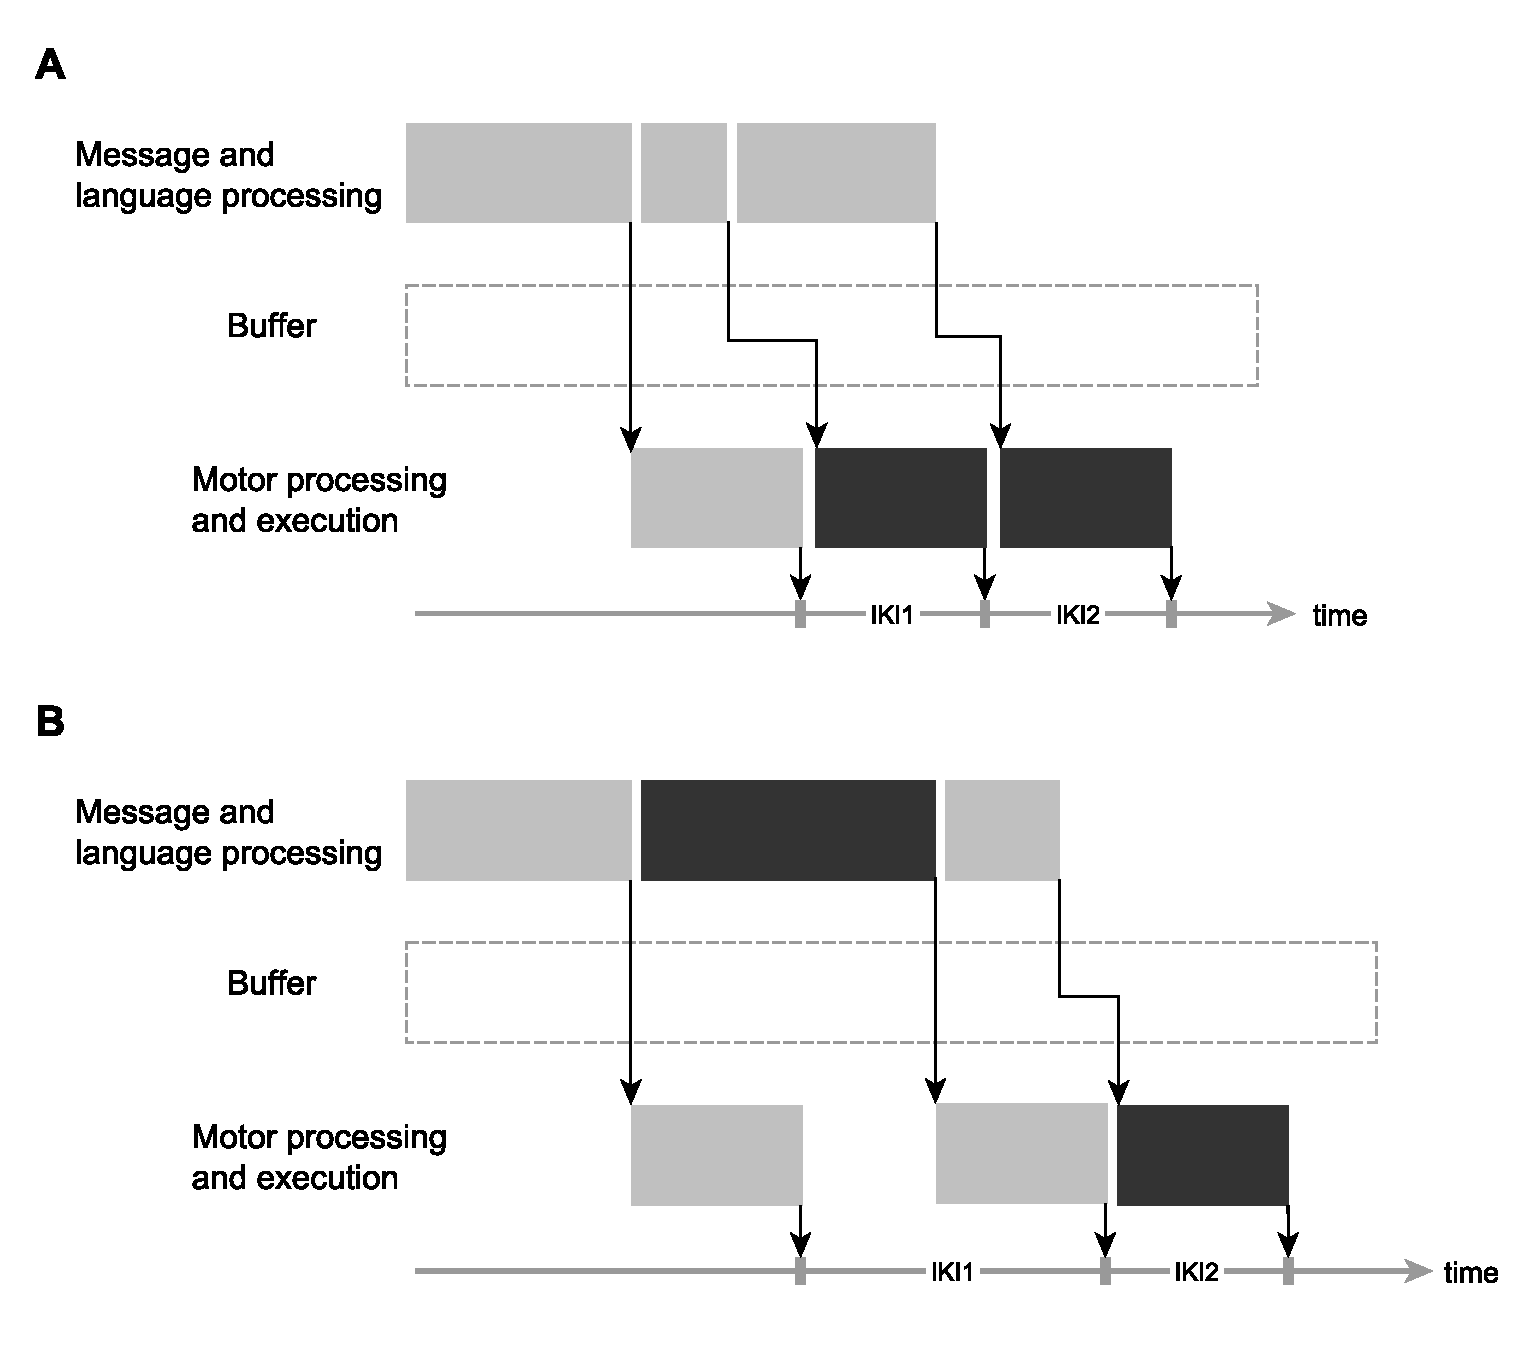
\includegraphics{figures/cascade_figure.pdf}
  \caption{Illustration of a parallel theory of text production.}
  \label{fig:model}
\end{figure}

In both cases the specific processing that is responsible for determining interkey interval is shown in black. Figure \ref{fig:model}A shows the case where upstream processing runs faster than, and therefore ahead of, motor execution. Message and language processing provides necessary information to the execution processes in advance of (or at exactly the same time as) when it can be used. In this case interkey intervals -- both IKI1 and IKI2 -- are determined just by the time taken to prepare and execute the keystroke. It is entirely unaffected by the duration of upstream processing. Figure \ref{fig:model}B shows the case where upstream processes deliver information to motor processes at a rate that lags behind that at which it could be potentially motor-planned and executed (i.e.~where \enquote{just in time} processing fails). This results in a delay in output -- a \enquote{hesitation} in our terminology. IKI1 in Figure \ref{fig:model}B is therefore longer than IKI1 in Figure \ref{fig:model}A. Just-in-time processing is then resumed, and IKI2 in Figure \ref{fig:model}B is of the same duration as the interkey intervals in Figure \ref{fig:model}A.

In the case where upstream processes run ahead of motor processing, the interkey interval is obviously determined just by the speed at which the writer can move their finger (can motor-plan and execute). The essential point that Figure \ref{fig:model} illustrates is that in the case where upstream processes lag behind motor output (Figure \ref{fig:model}B), the interkey interval is determined \emph{just} by time taken for upstream processing. Effects on the interkey interval are not additive. Interkey intervals are therefore determined by one of two entirely separate data-generating processes. This is the basis for our claim that a finite mixture of two distributions represents a statistical model of parallel processing.

\newpage

\hypertarget{statistical-models}{%
\section{Statistical models}\label{statistical-models}}

We implemented four statistical models using the Bayesian framework (e.g. Farrell \& Lewandowsky, 2018; Gelman et al., 2014; Lee \& Wagenmakers, 2014) to evaluate the serial or the parallel view. In other words, we used statistical models to map between keystroke data and the theoretically assumed cognitive process that underlies the generation of theses data. These models are presented in more detail in this section.

\hypertarget{single-distribution-gaussian-model}{%
\subsection{Single-distribution Gaussian model}\label{single-distribution-gaussian-model}}

Under the serial view, all planning relevant for the to-be-produced utterance must be completed prior to typing onset. The duration of the resulting interkey interval depends on, among others, psycholinguistic factors; i.e.~interkey intervals that are located before easily retrievable high-frequency words tend to be short; similar for words with fewer graphemes, syllables, and morphemes (Nottbusch et al., 2005; Roeser et al., 2019; Torrance et al., 2018). We can capture the variability associated with word-features by assuming that before-word interkey intervals can be described as coming from a normal (Gaussian) distribution that can be fully characterised by an unknown central tendency \(\mu\) of interkey intervals associated with word-level planning and a dispersion \(\sigma_\text{e}^2\), that captures the residual variance in the data that is not captured by the model. This can be expressed as \(\text{iki}_\text{before word} \sim \mathcal{N}(\mu, \sigma_\text{e}^2)\) where \(\text{iki}_\text{before word}\) are all interkey intervals immediately proceeding a word. Of importance is the estimated value of the central tendency parameter \(\mu\) representing in this case the average time needed to mentally prepare a word.

We can extend this simple model of word planning to other linguistic locations. Edges of larger linguistic units are typically understood as being associated with planning on higher levels. For example, at sentence boundaries, planning needs to happen for word-level properties -- which we captured before with the parameter \(\mu\) -- but also for higher level information such as what meaning it is that should be conveyed, which word to plan and output first, and potentially even dependencies of the sentence-initial noun (Nottbusch et al., 2007; Roeser et al., 2019). We can capture factors that we assume to impact interkey intervals by decomposing \(\mu\) into the general form \(\mu = \alpha + \beta \times \text{x}\). For example, to capture the additional planning needed at sentence boundaries we can add the predictor \(\text{x}_\text{sentence[0,1]}\) so that \(\mu = \alpha + \beta \times \text{x}_\text{sentence[0,1]}\). This states that when the value of \(\text{x}_\text{sentence}\) takes on 0, the equation reduces to \(\mu = \alpha\) which is then the average interkey interval for word boundaries but, when \(\text{x}_\text{sentence}\) takes on the value 1, the average interkey interval for word boundaries \(\alpha\) is incremented by a changed in the outcome variable of \(\beta\) msecs. The value of the \(\beta\) parameter represents, therefore, the additional planning necessary for sentences. The application of such a statistical model to the data therefore provides us with an estimate of the parameter value that can be used for statistical inference (e.g.~to determine whether there is evidence for a statistically meaningful difference for interkey intervals immediately proceeding words vs sentences).

We implemented such a model -- a standard Gaussian mixed-effects model -- as described in equation \ref{eq:unimodgaus}. This model assumes that interkey intervals \(\text{iki}_i\) with \(i \in 1 \ldots N\) where \(N\) is the total number of interkey intervals come from a Gaussian distribution with a mean \(\mu\),

\begin{equation}
\begin{aligned}
\label{eq:unimodgaus}
\text{iki}_i \sim\text{ } & \mathcal{N}(\mu_i, \sigma_\text{e}^2)\\
\text{where: } & \mu_i = \beta_\text{location[i]} + u_\text{participant[i]}\\
& u_\text{participant[i]} \sim \mathcal{N}(0, \sigma_\text{p}^2)\\
\text{constraint: } & \sigma_\text{e}^2, \sigma_\text{p}^2>0
\end{aligned}
\end{equation}

which is a linear function of the \(i^\text{th}\) transition location (we used there levels: before sentence, before word, within word) captured by \(\beta_\text{location}\), and the random-intercept term \(u_\text{participant}\) which is constrained to come from a normal distribution with a mean of 0 and the standard deviation \(\sigma_\text{p}^2\). For the random-intercept term, \(\text{participant[i]}\) is the participant associated with the \(i^\text{th}\) interkey interval. The posterior of \(u_\text{participant}\) is therefore the difference between the posterior interkey-interval estimate of each participant (i.e.~a positive value indicates that a participant is slower than average; a negative value indicates that a participant is faster than average) and allows to capture the fact that some writers are faster and other writers are slower. Importantly this model returns posterior probability distributions with interkey-interval estimates for each \(\beta\), one for each transition location.

Standard-deviation parameters were constrained to be positive because standard deviations can, by definition, never be negative.

\hypertarget{single-distribution-log-gaussian-model}{%
\subsection{Single-distribution log-Gaussian model}\label{single-distribution-log-gaussian-model}}

The previous model assumes a Gaussian probability function as the underlying data-generating process. The model presented in this section is identical to the previous model but instead of assuming a Gaussian probability function, we assume that the process that generates the follows a log-normal (log-Gaussian) distribution.

There are, at least, two reason for why a log-Gaussian distribution is more appropriate than a standard Gaussian: (1) the log-Gaussian have a natural lower bound. This is a desirable property because the distance between two subsequent keystroke events is by definition positive. The lower bound of the distribution of interkey intervals is delimited by a writer's ability to move their fingers and keyboard polling. (2) the log-scale is known to be a better match for data from human motor behaviour and response time data than the normal distribution (Baayen, 2008; Wagenmakers \& Brown, 2007). This is because in a Gaussian distribution the distance between adjacent units is linear. In other words a difference of 25 msecs is the same between 100 and 125 msecs as between 5 secs and 5,025 msecs. This does not map onto the psychological interpretation for short and long interkey intervals. For example effects that result from difficulty on the motor level (e.g.~executing familiar key combinations such as \emph{ng} compared to \emph{gn}) are typically smaller than differences that are due to higher levels of processing (e.g.~struggling to retrieve a word in an L1 or L2). In other words, an effect of 25 msecs is relatively large in the context of lower-level motor events but small in the context of higher-level cognitive activity such as planning what to say next. Log-Gaussian distributions are a natural way of translating a linear scale to an exponential scale so that a 25 msecs difference on the lower end (motor activity) is more psychologically meaningful than a 25 msecs difference on the upper end of the distribution interkey intervals (retrieving words, planning contents).

This model can be described as in equation \ref{eq:unimodloggaus} in which the distribution \(\mathcal{N}()\) was replaced by \(\log\mathcal{N}()\) to represent a log-normal distribution.

\begin{equation}
\begin{aligned}
\label{eq:unimodloggaus}
\text{iki}_i \sim\text{ } & \log\mathcal{N}(\mu_i, \sigma_\text{e}^2) \\
\text{where: } &
\mu_i = \beta_\text{location[i]} + u_\text{participant[i]}\\
& u_\text{participant[i]} \sim \mathcal{N}(0, \sigma_\text{p}^2) \\
\text{constraint: } & \sigma_\text{e}^2, \sigma_\text{p}^2>0
\end{aligned}
\end{equation}

\hypertarget{single-distribution-unequal-variance-log-gaussian-model}{%
\subsection{Single-distribution unequal-variance log-Gaussian model}\label{single-distribution-unequal-variance-log-gaussian-model}}

The third model is identical to the model presented in the previous section but relaxed the equal-variance assumption associated with transition location. In particular the previous models assumed that the variances associated with each transition location were identical. This assumption does however not fit with what we know about data from human motor behaviour. Longer latencies are known to be associated with a larger variance for human motor behaviour (Schöner, 2002; Wagenmakers \& Brown, 2007; Wing \& Kristofferson, 1973). For interkey intervals pauses at edges of larger linguistic units can therefore be assumed to be associated with a larger variance. In equation \ref{eq:unimoduv}, we introduced this assumption by allowing the standard deviations \(\sigma_{e_\text{location}}^2)\) to vary by transition location.

\begin{equation}
\begin{aligned}
\label{eq:unimoduv}
\text{iki}_i \sim\text{ } & \log\mathcal{N}(\mu_i, \sigma_{e_\text{location[i]}}^2) \\
\text{where: } & \mu_i = \beta_\text{location[i]} + u_\text{participant[i]}\\
 & u_\text{participant[i]} \sim \mathcal{N}(0, \sigma_\text{p}^2) \\
 \text{constraint: } & \sigma_\text{e}^2, \sigma_\text{p}^2>0
\end{aligned}
\end{equation}

\hypertarget{two-distribution-log-gaussian-mixture-model}{%
\subsection{Two-distribution log-Gaussian mixture model}\label{two-distribution-log-gaussian-mixture-model}}

The following model is an extension of the previous single-distribution model. In contrast to the models introduced for the serial view of writing, the parallel view assumes that planning occurs while previously planned language units are being executed in writing. For the model presented in this section we removed the constraint that all planning must be completed before writing onset. In other words, instead of assuming that different linguistic edges shift the distribution over average interkey intervals towards larger values -- as in the previous models -- the parallel view assumes the frequency of observing a hesitant intekey interval and the size of this hesitation depends on text location of the key transition. This was achieved by introducing the assumption that interkey intervals come from a weighted combination (i.e.~mixture) of two distributions associated with two different states:

\begin{enumerate}
\def\labelenumi{\arabic{enumi}.}
\item
  Activation flows into keystrokes without interruption. These fluent interkey intervals are merely constrained by a writer's ability to move their fingers and were captured by \(\beta\) in equation \ref{eq:bimodcon}. In other words, \(\beta\) represents the average typing speed for fluent transitions between keys. Note that the \(\beta\) parameter is represented in both log-Gaussian distributions in equation \ref{eq:bimodcon}.
\item
  Interruptions in the activation flow from higher to lower levels result in longer keystroke intervals when information was not available in time, for example when competition occurs during lexical retrieval or when its orthographic representation was not easily available. The slowdown for these hesitant transitions is captured by \(\delta\) in the first line of equation \ref{eq:bimodcon}. This \(\delta\) parameter was constrained to be positive and added to the distribution of fluent key transitions \(\beta\). It therefore represents the magnitude of the slowdown associated with hesitant transitions. The slowdown \(\delta\) was allowed to vary by transition locations because hesitations at larger linguistic units are more likely to be associated with higher level planning which may delay output.
\end{enumerate}

The first line of equation \ref{eq:bimodcon} represents the distribution of hesitant interkey intervals; the second line represents fluent interkey intervals.

\begin{equation}
\begin{aligned}
\label{eq:bimodcon}
\text{iki}_{i} \sim\text{ } & \theta_\text{location[i], participant[i]} \times \log\mathcal{N}(\beta + \delta_\text{location[i]} + u_\text{participant[i]}, \sigma_{e'_\text{location[i]}}^2) + \\
  & (1 - \theta_\text{location[i], participant[i]}) \times \log\mathcal{N}(\beta + u_\text{participant[i]}, \sigma_{e_\text{location[i]}}^2)\\
\text{where: } & u_\text{participant[i]} \sim \mathcal{N}(0, \sigma_\text{p}^2) \\
\text{constraint: } & \delta, \sigma_{e}^2, \sigma_\text{e'}^2, \sigma_\text{p}^2>0\\
        & \sigma_{e'}^2 > \sigma_{e}^2\\
        & 0 < \theta < 1
\end{aligned}
\end{equation}

These two distributions are associated with the mixing weight \(\theta\) which must be larger than 0 and smaller than 1. \(\theta\) is parameterised to represent the weighting of the distribution in the first line, hence representing the \emph{hesitation probability}. This probability is inversely related to the mixing weight of the distribution of short interkey intervals by \(1-\theta\) as the weights of both distributions must sum to 1. In line with the literature discussed in the introduction, we assume that the hesitation probability is likely to vary across linguistic locations. As hesitation frequency is subject to individual differences and writing style (and skills), we also assumed that some participants are more and others are less likely to hesitate at certain transition locations (Van Waes et al., 2021).

Lastly, we carried over the unequal variance assumption and let the standard deviations \(\sigma_{e'}^2\) and \(\sigma_{e}^2\) vary by transition location. We constrained the standard deviations so that \(\sigma_{e'}\) which is associated with the distribution of hesitant interkey intervals is larger than the standard deviation associated with fluent transitions \(\sigma_e\) for reasons discussed above.

\newpage

\hypertarget{fit-to-data}{%
\section{Fit to data}\label{fit-to-data}}

Model fit was assessed by testing to what extent data simulated from the model match the observed data. From each model we obtained 50 simulations (predictions). Simulated and observed data are visualised in Figure \ref{fig:prediction}. Data predicted by the mixture model were substantially more similar to the observed data compared to any of the single-distribution models. The worse fit was observed for the single-distribution Gaussian model which predicted a larger number of negative keystroke intervals.

\begin{figure}

{\centering \includegraphics{figures/fitplots} 

}

\caption{Predicted data (50 simulations in each cell) in red compared to interkey interval data shown in black shown by model and datasets. Better fit i shown on the left and weaker fit is shown on the right. X-axes were truncated at 2 secs.}\label{fig:prediction}
\end{figure}

\newpage

\hypertarget{key-combination-effect}{%
\section{Key-combination effect}\label{key-combination-effect}}

Interkey intervals at before sentence location either did (PLanTra, LIFT) scope over both the shift key and the character following the shift key or included only the first key following a the space immediately proceeding a sentence (CATO, C2L1, SPL2, GE2). In other words, the interkey interval before sentences are sum of two interkey intervals in the PLanTra and LIFT data, namely \texttt{\_\^{}{[}shift{]}\^{}C}, where \texttt{\^{}} represents a transition between keys, consists only of one interkey interval, namely \texttt{\_\^{}{[}shift{]}}, in the remaining datasets. Therefore, differences in hesitation patterns across datasets for transitions immediately proceeding a sentence could be explained without reference to edges of linguistic units.

Therefore we tested to what extent the inclusion of one additional interkey interval at sentence boundaries affected the hesitation results. We used the SPL2 data for this comparison and calculated intervals including and excluding the keystroke following a sentence-initial shift press. Although we modelled all transition locations, we present only before-sentence transitions as there was, as one would expect, no difference for before and within-word interkey intervals. The results of this comparison can be found in Table \ref{tab:shiftcellmeans} (only for the data from participants writing in their first language).

\begin{center}
\begin{ThreePartTable}

\begin{TableNotes}[para]
\normalsize{\textit{Note.} PIs are probability intervals. BF is the evidence in favour of the alternative hypothesis over the null hypothesis.}
\end{TableNotes}

\footnotesize{

\begin{longtable}{llrrr}\noalign{\getlongtablewidth\global\LTcapwidth=\longtablewidth}
\caption{\label{tab:shiftcellmeans}Mixture model estimates for interkey interval immediately preceding a sentence. Cellmeans are shown for interkey intervals that do and do not include the interkey interval following a sentence-initial shift key press. Hesitation duration is shown in mseecs along with the hesitation probability. The difference due to the additional keystoke is shown fo the hesitation duration (log scale) and hesitation probability (logit scale); 95\% PIs are shown in brackets.}\\
\toprule
Model parameter & \multicolumn{1}{c}{\_\textasciicircum{}[shift]\textasciicircum{}C} & \multicolumn{1}{c}{\_\textasciicircum{}[shift]} & \multicolumn{1}{c}{Difference} & \multicolumn{1}{c}{BF}\\
\midrule
\endfirsthead
\caption*{\normalfont{Table \ref{tab:shiftcellmeans} continued}}\\
\toprule
Model parameter & \multicolumn{1}{c}{\_\textasciicircum{}[shift]\textasciicircum{}C} & \multicolumn{1}{c}{\_\textasciicircum{}[shift]} & \multicolumn{1}{c}{Difference} & \multicolumn{1}{c}{BF}\\
\midrule
\endhead
Fluent interkey intervals & 156 [145, 169] & 159 [147, 172] & -0.02 [-0.13, 0.09] & 0.06\\
Hesitation duration & 1,324 [1,186, 1,470] & 1,440 [1,236, 1,662] & -0.06 [-0.21, 0.09] & 0.11\\
Hesitation probability & 1.00 [.99, 1.00] & .78 [.69, .86] & 4.91 [3.68, 6.35] & > 100\\
\bottomrule
\addlinespace
\insertTableNotes
\end{longtable}

}

\end{ThreePartTable}
\end{center}

The duration of fluent and hesitant interkey intervals was not affected by whether or not the sentence-initial transition include the character following the shift key. However, we found strong evidence for an increased hesitation probability when the before-sentence interkey interval included the character following the shift key. Notably, the hesitation probability approached ceiling when the interkey interval following the shift key was added. In other words, the mixture model identified almost all before-sentence transitions as being hesitant as they -- in the majority of cases -- included two keystrokes while interkey intervals for all other transition locations -- and therefore the majority of the data -- did not.

\newpage

\hypertarget{l2-effect-spl2}{%
\section{L2 effect (SPL2)}\label{l2-effect-spl2}}

For the SPL2 data we calculated the L2 effect (i.e.~the effect of writing in L2 or L1). The results can be found in Table \ref{tab:l2effect}. The results show longer hesitation duration and more hesitations across all transition locations when writing in L2. Only within-word transitions showed negligible evidence for more or longer hesitations.

\begin{table}[tbp]

\begin{center}
\begin{threeparttable}

\caption{\label{tab:l2effect}Mixture model estimates for language effect. Cellmeans are shown for the hesitation duration and for the probability of hesitant interkey intervals for texts produced in the writer's L1 and L2. Language differences are shown for the hesitation duration (log scale) and the hesitation probability (logit scale); 95\% PIs in brackets.}

\small{

\begin{tabular}{lrrrr}
\toprule
Transition location & \multicolumn{1}{c}{L1} & \multicolumn{1}{c}{L2} & \multicolumn{1}{c}{Difference} & \multicolumn{1}{c}{BF}\\
\midrule
Hesitation duration &  &  &  & \\
\ \ \ before sentence & 1,440 [1,236, 1,662] & 1,961 [1,710, 2,240] & 0.31 [0.17, 0.45] & > 100\\
\ \ \ before word & 448 [405, 495] & 719 [656, 788] & 0.47 [0.39, 0.55] & > 100\\
\ \ \ within word & 279 [210, 384] & 362 [310, 422] & 0.27 [-0.07, 0.55] & 0.68\\
Hesitation probability &  &  &  & \\
\ \ \ before sentence & .78 [.69, .86] & .92 [.87, .96] & 1.23 [0.52, 1.97] & > 100\\
\ \ \ before word & .51 [.41, .62] & .89 [.83, .93] & 2.02 [1.4, 2.66] & > 100\\
\ \ \ within word & .04 [.02, .07] & .15 [.10, .22] & 1.52 [0.78, 2.29] & > 100\\
\bottomrule
\addlinespace
\end{tabular}

}

\begin{tablenotes}[para]
\normalsize{\textit{Note.} PIs are probability intervals. BF is the evidence in favour of the alternative hypothesis over the null hypothesis.}
\end{tablenotes}

\end{threeparttable}
\end{center}

\end{table}

\newpage

\hypertarget{masking-effect-cato-ge2}{%
\section{Masking effect (CATO, GE2)}\label{masking-effect-cato-ge2}}

Studies associated with the CATO and GE2 datasets investigated to what extent hiding (masking) previously written text from the reader affects keystroke behaviour. Mixture model results for the masking effect are shown in Table \ref{tab:maskingeffect}. There is some evidence that when the text was masked dylexic writers hesitated longer before starting to type sentences. Evidence for all other comparisons was negligible.

\begin{landscape}

\begin{center}
\begin{ThreePartTable}

\begin{TableNotes}[para]
\normalsize{\textit{Note.} PIs are probability intervals. BF is the evidence in favour of the alternative hypothesis over the null hypothesis.}
\end{TableNotes}

\footnotesize{

\begin{longtable}{lllrrrr}\noalign{\getlongtablewidth\global\LTcapwidth=\longtablewidth}
\caption{\label{tab:maskingeffect}Mixture-model estimates for masking effect. Cellmeans are shown for the masked and unmasked writing task for hesitation duration (in msecs) and hesitation probability. The masking effect is shown on the log scale for durations and on the logit scale for probabilities; 95\% PIs in brackets.}\\
\toprule
Transition location & \multicolumn{1}{c}{Dataset} & \multicolumn{1}{c}{Group} & \multicolumn{1}{c}{Unmasked} & \multicolumn{1}{c}{Masked} & \multicolumn{1}{c}{Difference} & \multicolumn{1}{c}{BF}\\
\midrule
\endfirsthead
\caption*{\normalfont{Table \ref{tab:maskingeffect} continued}}\\
\toprule
Transition location & \multicolumn{1}{c}{Dataset} & \multicolumn{1}{c}{Group} & \multicolumn{1}{c}{Unmasked} & \multicolumn{1}{c}{Masked} & \multicolumn{1}{c}{Difference} & \multicolumn{1}{c}{BF}\\
\midrule
\endhead
Hesitation duration &  &  &  &  &  & \\
\ \ \ before sentence & CATO & dyslexic & 2,423 [1,731, 3,302] & 1,871 [1,428, 2,398] & -0.25 [-0.64, 0.13] & 0.44\\
\ \ \ before sentence & CATO & non dyslexic & 1,924 [1,429, 2,518] & 1,693 [1,323, 2,134] & -0.12 [-0.47, 0.22] & 0.23\\
\ \ \ before sentence & GE2 & non dyslexic & 1,282 [1,108, 1,469] & 1,575 [1,369, 1,796] & 0.21 [0.05, 0.36] & 2.59\\
\ \ \ before word & CATO & dyslexic & 635 [590, 683] & 598 [553, 644] & -0.06 [-0.13, 0.01] & 0.14\\
\ \ \ before word & CATO & non dyslexic & 536 [497, 579] & 518 [480, 558] & -0.04 [-0.11, 0.04] & 0.06\\
\ \ \ before word & GE2 & non dyslexic & 520 [476, 567] & 536 [492, 584] & 0.03 [-0.05, 0.11] & 0.05\\
\ \ \ within word & CATO & dyslexic & 469 [356, 593] & 368 [305, 445] & -0.24 [-0.52, 0.06] & 0.57\\
\ \ \ within word & CATO & non dyslexic & 600 [434, 787] & 583 [420, 784] & -0.03 [-0.42, 0.38] & 0.2\\
\ \ \ within word & GE2 & non dyslexic & 339 [261, 438] & 367 [290, 466] & 0.08 [-0.24, 0.4] & 0.19\\
Hesitation probability &  &  &  &  &  & \\
\ \ \ before sentence & CATO & dyslexic & .60 [.38, .79] & .80 [.60, .93] & 0.2 [-0.06, 0.46] & 0.45\\
\ \ \ before sentence & CATO & non dyslexic & .55 [.34, .76] & .68 [.47, .84] & 0.13 [-0.16, 0.4] & 0.21\\
\ \ \ before sentence & GE2 & non dyslexic & .88 [.82, .93] & .90 [.85, .94] & 0.16 [-0.46, 0.79] & 0.36\\
\ \ \ before word & CATO & dyslexic & .75 [.64, .85] & .72 [.59, .82] & -0.04 [-0.19, 0.12] & 0.09\\
\ \ \ before word & CATO & non dyslexic & .64 [.51, .75] & .62 [.49, .74] & -0.02 [-0.19, 0.16] & 0.09\\
\ \ \ before word & GE2 & non dyslexic & .47 [.40, .54] & .45 [.38, .52] & -0.06 [-0.46, 0.35] & 0.21\\
\ \ \ within word & CATO & dyslexic & .07 [.03, .12] & .11 [.06, .19] & 0.05 [-0.02, 0.13] & 0.08\\
\ \ \ within word & CATO & non dyslexic & .03 [.02, .06] & .03 [.02, .06] & 0 [-0.03, 0.03] & 0.01\\
\ \ \ within word & GE2 & non dyslexic & .05 [.03, .08] & .04 [.03, .06] & -0.29 [-0.88, 0.28] & 0.48\\
\bottomrule
\addlinespace
\insertTableNotes
\end{longtable}

}

\end{ThreePartTable}
\end{center}
\end{landscape}

\newpage

\hypertarget{posterior-parameter-estimates}{%
\section{Posterior parameter estimates}\label{posterior-parameter-estimates}}

\begin{figure}[!htb]
\centering
\includegraphics{figures/psplots1constr.pdf}
\caption{Distribution of posterior parameter estimates with 95\% probability intervals (PI). Fluent interkey intervals and hesitation durations are shown in msecs; probability of hesitations is the proportion of hesitant interkey intervals.}
\end{figure}
\newpage
\begin{figure}[!htb]
\ContinuedFloat
\captionsetup{list=off,format=cont}
\centering
\includegraphics{figures/psplots2constr.pdf}
\label{fig:fullps1}
\caption{Distribution of posterior parameter estimates with 95\% probability intervals (PI). Fluent interkey intervals and hesitation durations are shown in msecs; probability of hesitations is the proportion of hesitant interkey intervals.}

\end{figure}

\newpage

\hypertarget{pre-post-test-plantra}{%
\section{Pre-post test (PLanTra)}\label{pre-post-test-plantra}}

The pre-post test effect for the PLanTra dataset is reported in Table \ref{tab:retesteffect}. Evidence for all comparisons was negligible.

\begin{center}
\begin{ThreePartTable}

\begin{TableNotes}[para]
\normalsize{\textit{Note.} PIs are probability intervals. BF is the evidence in favour of the alternative hypothesis over the null hypothesis.}
\end{TableNotes}

\footnotesize{

\begin{longtable}{lrrrr}\noalign{\getlongtablewidth\global\LTcapwidth=\longtablewidth}
\caption{\label{tab:retesteffect}Mixture model estimates for post-test effect. Cellmeans are shown for pre and post-test for the duration of hesitant interkey intervals in msecs and its probability. Differences are shown on the log scale for hesitation duration and on the logit scale for the hesitation probability; 95\% PIs in brackets.}\\
\toprule
Transition location & \multicolumn{1}{c}{Pre-test} & \multicolumn{1}{c}{Post-test} & \multicolumn{1}{c}{Difference} & \multicolumn{1}{c}{BF}\\
\midrule
\endfirsthead
\caption*{\normalfont{Table \ref{tab:retesteffect} continued}}\\
\toprule
Transition location & \multicolumn{1}{c}{Pre-test} & \multicolumn{1}{c}{Post-test} & \multicolumn{1}{c}{Difference} & \multicolumn{1}{c}{BF}\\
\midrule
\endhead
Hesitation duration &  &  &  & \\
\ \ \ before sentence & 1,034 [875, 1,210] & 1,064 [893, 1,257] & -0.03 [-0.23, 0.17] & 0.1\\
\ \ \ before word & 593 [544, 645] & 589 [540, 643] & 0.01 [-0.08, 0.1] & 0.05\\
\ \ \ within word & 399 [333, 480] & 424 [353, 509] & -0.06 [-0.3, 0.18] & 0.14\\
Hesitation probability &  &  &  & \\
\ \ \ before sentence & .58 [.50, .66] & .54 [.47, .62] & 0.15 [-0.26, 0.58] & 0.27\\
\ \ \ before word & .56 [.50, .61] & .49 [.43, .55] & 0.27 [-0.04, 0.59] & 0.72\\
\ \ \ within word & .11 [.08, .14] & .09 [.07, .12] & 0.13 [-0.27, 0.54] & 0.26\\
\bottomrule
\addlinespace
\insertTableNotes
\end{longtable}

}

\end{ThreePartTable}
\end{center}

\newpage

\hypertarget{genre-effect-lift}{%
\section{Genre effect (LIFT)}\label{genre-effect-lift}}

From the LIFT data, we assessed differences between genres, i.e.~writing an informative as opposed to argumentative text. Results are shown in Table \ref{tab:genreeffect}. Cellmeans and differences were average across writing topic. Evidence for all comparisons was negligible.

\begin{center}
\begin{ThreePartTable}

\begin{TableNotes}[para]
\normalsize{\textit{Note.} PIs are probability intervals. BF is the evidence in favour of the alternative hypothesis over the null hypothesis.}
\end{TableNotes}

\footnotesize{

\begin{longtable}{lrrrr}\noalign{\getlongtablewidth\global\LTcapwidth=\longtablewidth}
\caption{\label{tab:genreeffect}Mixture-model estimates for genre effect. Cellmeans for hesitation duration (in msecs) and the probability of hesitant transitions are shown for argumentative and informative texts. The genre effect is shown on the log scale for hesitationn durations and on the logit scale for the probability of hesitant transitions; 95\% PIs in brackets.}\\
\toprule
Transition location & \multicolumn{1}{c}{Argumentative} & \multicolumn{1}{c}{Informative} & \multicolumn{1}{c}{Difference} & \multicolumn{1}{c}{BF}\\
\midrule
\endfirsthead
\caption*{\normalfont{Table \ref{tab:genreeffect} continued}}\\
\toprule
Transition location & \multicolumn{1}{c}{Argumentative} & \multicolumn{1}{c}{Informative} & \multicolumn{1}{c}{Difference} & \multicolumn{1}{c}{BF}\\
\midrule
\endhead
Hesitation duration &  &  &  & \\
\ \ \ before sentence & 524 [451, 606] & 562 [481, 656] & -0.07 [-0.33, 0.19] & 0.16\\
\ \ \ before word & 438 [400, 479] & 435 [398, 476] & 0.01 [-0.15, 0.16] & 0.09\\
\ \ \ within word & 351 [269, 458] & 397 [306, 513] & -0.12 [-0.6, 0.36] & 0.29\\
Hesitation probability &  &  &  & \\
\ \ \ before sentence & .35 [.28, .43] & .34 [.27, .42] & 0.05 [-0.57, 0.73] & 0.36\\
\ \ \ before word & .46 [.39, .54] & .48 [.41, .55] & -0.05 [-0.51, 0.44] & 0.25\\
\ \ \ within word & .07 [.05, .10] & .07 [.05, .10] & -0.02 [-0.81, 0.76] & 0.46\\
\bottomrule
\addlinespace
\insertTableNotes
\end{longtable}

}

\end{ThreePartTable}
\end{center}

\newpage

\hypertarget{transition-location-effect-1}{%
\section{Transition location effect}\label{transition-location-effect-1}}

\begin{center}
\begin{ThreePartTable}

\begin{TableNotes}[para]
\normalsize{\textit{Note.} PI = probability intervals. BF = evidence in favour of the alternative hypothesis over the null hypothesis.}
\end{TableNotes}

\footnotesize{

\begin{longtable}{lrrrr}\noalign{\getlongtablewidth\global\LTcapwidth=\longtablewidth}
\caption{\label{tab:loceffectcon}Transition-location effect. Differences are shown for the hesitation duration (log scale) and the hesitation probability (logit scale); 95\% PIs in brackets.}\\
\toprule
 & \multicolumn{2}{c}{Hesitation duration} & \multicolumn{2}{c}{Hesitation probability} \\
\cmidrule(r){2-3} \cmidrule(r){4-5}
Comparison & Est. [95\% PIs] & BF & Est. [95\% PIs] & BF\\
\midrule
\endfirsthead
\caption*{\normalfont{Table \ref{tab:loceffectcon} continued}}\\
\toprule
 & \multicolumn{2}{c}{Hesitation duration} & \multicolumn{2}{c}{Hesitation probability} \\
\cmidrule(r){2-3} \cmidrule(r){4-5}
Comparison & Est. [95\% PIs] & BF & Est. [95\% PIs] & BF\\
\midrule
\endhead
\textbf{C2L1} &  &  &  & \\
\ \ \ before sentence vs word & 0.24 [0.02, 0.48] & 1.11 & 0.44 [-0.56, 1.66] & 0.68\\
\ \ \ before vs within word & -0.03 [-0.14, 0.09] & 0.07 & 3.95 [3.54, 4.38] & > 100\\
\textbf{CATO (non-dyslexic, unmasked)} &  &  &  & \\
\ \ \ before sentence vs word & 1.27 [0.98, 1.55] & > 100 & -0.36 [-1.41, 0.69] & 0.67\\
\ \ \ before vs within word & -0.1 [-0.38, 0.21] & 0.2 & 4.05 [3.2, 4.91] & > 100\\
\textbf{GE2 (unmasked)} &  &  &  & \\
\ \ \ before sentence vs word & 0.9 [0.76, 1.04] & > 100 & 2.15 [1.6, 2.75] & > 100\\
\ \ \ before vs within word & 0.44 [0.17, 0.69] & 26.78 & 2.76 [2.24, 3.28] & > 100\\
\textbf{LIFT} &  &  &  & \\
\ \ \ before sentence vs word & 0.21 [-0.05, 0.48] & 0.5 & -0.53 [-1.04, 0.08] & 1.61\\
\ \ \ before vs within word & 0.17 [-0.32, 0.53] & 0.41 & 2.48 [1.81, 3.22] & > 100\\
\textbf{PLanTra} &  &  &  & \\
\ \ \ before sentence vs word & 0.57 [0.4, 0.74] & > 100 & 0.16 [-0.25, 0.57] & 0.28\\
\ \ \ before vs within word & 0.36 [0.16, 0.56] & 55.53 & 2.3 [1.9, 2.7] & > 100\\
\textbf{SPL2 (L1)} &  &  &  & \\
\ \ \ before sentence vs word & 1.17 [1.02, 1.3] & > 100 & 1.23 [0.59, 1.88] & > 100\\
\ \ \ before vs within word & 0.48 [0.16, 0.76] & 9.07 & 3.3 [2.56, 4.08] & > 100\\
\bottomrule
\addlinespace
\insertTableNotes
\end{longtable}

}

\end{ThreePartTable}
\end{center}

\newpage

\hypertarget{simulation}{%
\section{Simulation}\label{simulation}}

A possible concern with our results -- the substantially better predictive performance for two-distribution mixture models -- is that, in principle, as the mixture model has more parameters it might always outperform single-distribution models. We addressed this concern before by using cross-validation techniques for model comparison which prevent overfit by penalising models with more parameters. To further address this concern we evaluated models -- similar to the ones used in the main text -- for two sets of simulated data. Data were simulated using two random number generators, one that samples data from a single distribution and another that samples data from a weighted combination of two distributions. These simulated datasets allow us to test the predictive performance of our models in a context where we know the true underlying data generating process.

The first dataset was simulated from a weighted mixture of two log-normal distributions similar to the process described above (equation \ref{eq:bimodcon}). This process and the corresponding Bayesian model that we used to parameter estimation is summarised in equation \ref{eq:simmog}.

\begin{equation}
\begin{aligned}
\label{eq:simmog}
\text{y} \sim\text{ } & \theta \times \log\mathcal{N}(\beta + \delta, \sigma^2_1) +\\
& (1 - \theta) \times \log\mathcal{N}(\beta, \sigma^2_2)\\
\text{constraint: } & \delta, \sigma_\text{2}^2, \sigma_\text{1}^2>0\\
        & \sigma_{1}^2 > \sigma_{2}^2
\end{aligned}
\end{equation}

The equivalent Bayesian model is largely identical to the model used in the main text but does not assume different parameters for transition locations and does not include random effects for participants. This is because we neither simulated data for different transition locations (or other factors) or repeated measures for participants. The model assumes two data generating processes with each assuming a log-normal distribution with a mixing proportion \(\theta\). The distribution of smaller values has a mean \(\beta\) and a standard deviation \(\sigma^2_2\); the second distribution of larger values is constrained to have a mean that is \(\delta\) units larger than \(\beta\) and has a standard deviation \(\sigma^2_1\) larger than the distribution with the central tendency \(\beta\).

In R we can simulate data for equation \ref{eq:simmog} using the helper function below.

\begin{Shaded}
\begin{Highlighting}[]
\CommentTok{\# Function for a mixture of two log{-}Gaussians}
\NormalTok{molg }\OtherTok{\textless{}{-}} \ControlFlowTok{function}\NormalTok{(n, theta, mu1, mu2, sigma1, sigma2) \{}
\NormalTok{  y0 }\OtherTok{\textless{}{-}} \FunctionTok{rlnorm}\NormalTok{(n, }\AttributeTok{mean =}\NormalTok{ mu1, }\AttributeTok{sd =}\NormalTok{ sigma1)}
\NormalTok{  y1 }\OtherTok{\textless{}{-}} \FunctionTok{rlnorm}\NormalTok{(n, }\AttributeTok{mean =}\NormalTok{ mu2, }\AttributeTok{sd =}\NormalTok{ sigma2)}
\NormalTok{  mix }\OtherTok{\textless{}{-}} \FunctionTok{rbinom}\NormalTok{(n, }\AttributeTok{size =} \DecValTok{1}\NormalTok{, }\AttributeTok{prob =}\NormalTok{ theta)}
\NormalTok{  y }\OtherTok{\textless{}{-}}\NormalTok{ y0 }\SpecialCharTok{*}\NormalTok{ (}\DecValTok{1} \SpecialCharTok{{-}}\NormalTok{ mix) }\SpecialCharTok{+}\NormalTok{ y1 }\SpecialCharTok{*}\NormalTok{ mix }
\NormalTok{\}}

\NormalTok{N }\OtherTok{\textless{}{-}} \DecValTok{1000} \CommentTok{\# number of participants}
\NormalTok{beta }\OtherTok{\textless{}{-}} \DecValTok{5} \CommentTok{\# mean of fluent interkey intervals (in log)}
\NormalTok{delta }\OtherTok{\textless{}{-}} \DecValTok{1} \CommentTok{\# increment for hesitant interkey intervals (in log)}
\NormalTok{theta }\OtherTok{\textless{}{-}}\NormalTok{ .}\DecValTok{35} \CommentTok{\# proportion of hesitations}
\NormalTok{sigma }\OtherTok{\textless{}{-}} \FunctionTok{c}\NormalTok{(.}\DecValTok{25}\NormalTok{, .}\DecValTok{5}\NormalTok{) }\CommentTok{\# error variance}

\CommentTok{\# Simulate data from a mixture of two log{-}Gaussians}
\NormalTok{y }\OtherTok{\textless{}{-}} \FunctionTok{molg}\NormalTok{(}\AttributeTok{n =}\NormalTok{ N, }
          \AttributeTok{theta =}\NormalTok{ theta,}
          \AttributeTok{mu1 =}\NormalTok{ beta,}
          \AttributeTok{mu2 =}\NormalTok{ beta }\SpecialCharTok{+}\NormalTok{ delta,}
          \AttributeTok{sigma1 =}\NormalTok{ sigma[}\DecValTok{1}\NormalTok{],}
          \AttributeTok{sigma2 =}\NormalTok{ sigma[}\DecValTok{2}\NormalTok{])}
\end{Highlighting}
\end{Shaded}

A second dataset was simulated coming from a single log-normal distribution following equation \ref{eq:simuv}. An equivalent Bayesian model was implemented for parameter estimation.

\begin{equation}
\begin{aligned}
\label{eq:simuv}
\text{y} \sim\text{ }& \log\mathcal{N}(\beta, \sigma^2)\\
\text{constraint: } & \sigma^2>0
\end{aligned}
\end{equation}

Data following the distribution in equation \ref{eq:simuv} can be simulated using the following R code:

\begin{Shaded}
\begin{Highlighting}[]
\NormalTok{N }\OtherTok{\textless{}{-}} \DecValTok{1000} \CommentTok{\# number of participants}
\NormalTok{beta }\OtherTok{\textless{}{-}} \DecValTok{5} \CommentTok{\# population mean}
\NormalTok{sigma }\OtherTok{\textless{}{-}}\NormalTok{ .}\DecValTok{25} \CommentTok{\# error variance}

\CommentTok{\# Simulate data from a single log{-}normal distribution}
\NormalTok{y }\OtherTok{\textless{}{-}} \FunctionTok{rlnorm}\NormalTok{(}\AttributeTok{n =}\NormalTok{ N, }\AttributeTok{mean =}\NormalTok{ beta, }\AttributeTok{sd =}\NormalTok{ sigma)}
\end{Highlighting}
\end{Shaded}

Again, the Bayesian model corresponding to this process is a simplified version of the single-distribution model used in the main text. The model assumes a log-Gaussian distribution with a mean \(\beta\) and a standard deviation \(\sigma^2\).

Both simulated datasets are visualised in Figure \ref{fig:simdata}. The parameter values used for each of the two data simulations can be seen in Table \ref{tab:simparam}. Parameter values were chosen so that the simulated data are distributed roughly similar to interkey interval data.

\begin{figure}

{\centering \includegraphics{manuscript_files/figure-latex/simdata-1} 

}

\caption{Data simulated with a two-distribution (yellow) and a single-distribution (grey) random data-generating process. The x-axis showing the outcome y was log-scaled for visibility.}\label{fig:simdata}
\end{figure}

For each of these two datasets we simulated 1,000 observations. We fitted 2 models -- the two-distribution mixture model and the single-distribution model described above -- for each dataset. Models were run with 3 chains, with each 6,000 iterations of which 3,000 iterations were discarded as warmup samples. Estimates with 95\% probability intervals are shown in Table \ref{tab:simparam}. True and estimated parameter values are shown for each data generating process and Bayesian model. Both models successfully uncovered the model parameters for the datasets simulated with the corresponding underlying process, but less so when the model was applied to the data generated with the other incorrect underlying process.

\begin{table}[tbp]

\begin{center}
\begin{threeparttable}

\caption{\label{tab:simparam}Uncovered parameter estimates with 95\% probability intervals (PI) and true parameter values for each simulated dataset by model.}

\begin{tabular}{lrr}
\toprule
 & \multicolumn{2}{c}{Estimates with 95\% PIs} \\
\cmidrule(r){2-3}
Parameter with true value & \multicolumn{1}{c}{Two-distribution data} & \multicolumn{1}{c}{Single-distribution data}\\
\midrule
Two-distribution model &  & \\
\ \ \ $\beta = 5$ & 5.02 [4.99, 5.04] & 4.93 [4.76, 5.01]\\
\ \ \ $\delta = 1$ & 1.04 [0.92, 1.14] & 0.13 [0.01, 0.3]\\
\ \ \ $\theta = .35$ & .33 [.28, .39] & .54 [.11, .92]\\
\ \ \ $\sigma^2_1 = 0.25$ & 0.25 [0.23, 0.27] & 0.22 [0.16, 0.25]\\
\ \ \ $\sigma^2_2 = 0.5$ & 0.49 [0.42, 0.57] & 0.25 [0.22, 0.3]\\
Single-distribution model &  & \\
\ \ \ $\beta = 5$ & 5.35 [5.32, 5.39] & 5 [4.99, 5.02]\\
\ \ \ $\sigma = 0.25$ & 0.6 [0.57, 0.63] & 0.25 [0.24, 0.26]\\
\bottomrule
\end{tabular}

\end{threeparttable}
\end{center}

\end{table}

We used leave-one-out cross-validation to compare the predictive performance of the two models for each data-generating process. Model comparisons can be found in Table \ref{tab:loossim}. For the data generated with a two-distribution mixture process, the mixture model shows a substantially higher predictive performance. In fact, the mixture model's predictive performance is 11.6 standard errors higher compared to the single-distribution model. However, the mixture model showed a slightly lower predictive performance (i.e.~a difference of 0.77 standard errors) for the single-process data. Thus, the single distribution model is the more parsimonious choice for the single-distribution data. These results rule out the possibility that mixture models always lead to higher predictive performance.

\begin{table}[tbp]

\begin{center}
\begin{threeparttable}

\caption{\label{tab:loossim}Model comparisons by dataset. The top row shows the models with the highest predictive performance for each data generating process. Standard error is shown in parentheses.}

\begin{tabular}{lrr}
\toprule
Model & \multicolumn{1}{c}{$\Delta\widehat{elpd}$} & \multicolumn{1}{c}{$\widehat{elpd}$}\\
\midrule
Data: Two-distribution mixture process &  & \\
\ \ \ Two-distribution mixture model & -- & -6,068 (41)\\
\ \ \ Single-distribution model & -191.3 (16.5) & -6,259 (38)\\
Data: Single-distribution process &  & \\
\ \ \ Single-distribution model & -- & -5,030 (24)\\
\ \ \ Two-distribution mixture model & -0.5 (0.7) & -5,030 (24)\\
\bottomrule
\addlinespace
\end{tabular}

\begin{tablenotes}[para]
\normalsize{\textit{Note.} $\widehat{elpd}$ = predictive performance indicated as expected log pointwise predictive density; $\Delta\widehat{elpd}$ = difference in predictive performance relative to the model with the highest predictive performance in the top row.}
\end{tablenotes}

\end{threeparttable}
\end{center}

\end{table}

\newpage


\end{document}
